\documentclass[11pt]{article}

\usepackage[T1]{fontenc}
\usepackage{amsmath,amssymb}
\usepackage{array}
\usepackage{booktabs}
\usepackage{geometry}
\usepackage{graphicx}
\usepackage{hyperref}
\usepackage{microtype}
\usepackage{placeins}
\usepackage{subcaption}
\usepackage{xcolor}

\geometry{margin=1in}
\graphicspath{{./}}
\hypersetup{
  colorlinks=true,
  linkcolor=blue!55!black,
  citecolor=blue!55!black,
  urlcolor=blue!55!black
}

\newcommand{\fro}{\mathrm{F}}
\newcommand{\RR}{\mathbb{R}}
\newcommand{\mat}[1]{\mathsf{#1}}
\newcommand{\vect}[1]{\boldsymbol{#1}}
\newcommand{\code}[1]{\texttt{#1}}

\title{Spectral Reduction in the One-Dimensional Particle-in-a-Box:\\
Verification, Dispersion, and Operator Identifiability}
\author{Eugene Joseph M. Ragasa\\
De La Salle University, Manila\\
\texttt{eugene.ragasa@dlsu.edu.ph}}
\date{Draft preprint --- \today}

\begin{document}
\maketitle

\begin{abstract}
The one-dimensional particle in a box provides a transparent setting for examining
what is preserved when a quantum Hamiltonian is discretized and reduced. We apply
centered finite differences on closed-interval grids and project the resulting
Hamiltonian onto its lowest-energy states, choosing the retained dimension from a
prescribed bound on omitted thermal probability. Because both the continuum and
discrete spectra are available in closed form, eigensolver accuracy, discretization
error, and projection error can be distinguished directly. The computed eigensystem
satisfies the finite spectral identities to roundoff. Fixed modes converge to their
continuum energies at second order, whereas modes whose wavelengths remain tied to the
grid scale retain a finite dispersion error under refinement. Residual comparisons
show that consistent compression preserves the zero-potential identity, unmatched
compression isolates the discarded kinetic sector, and changing the boundary closure
produces a boundary-localized residual rather than a potential. A model-class
comparison further shows that a known reduced matrix does not uniquely determine a
kinetic--potential decomposition. The familiar box model therefore provides a
controlled computational setting for understanding how grid resolution, subspace
selection, boundary conditions, and physical assumptions affect the interpretation
of reduced Hamiltonians. Separate numerical and machine-checked verification supports
these conclusions while remaining distinct from physical validation.
\end{abstract}

\noindent\textbf{Keywords:} particle in a box; spectral reduction; finite differences;
operator compression; convergence; identifiability; numerical verification

\section{Introduction}

The one-dimensional particle in a box is among the first exactly solvable models
encountered in quantum mechanics. Its energy levels, standing-wave eigenfunctions,
and boundary conditions make quantization visible with little mathematical overhead.
It is consequently well established as both a teaching model and a numerical
benchmark: software-assisted treatments visualize its states, while finite-difference
calculations recover its energies and wavefunctions
\cite{magalhaesVasconcelos2006,halpernGeGlendening2022}. That familiarity makes the
box useful for a less elementary question: what is actually preserved when a
continuum Hamiltonian is represented by a finite matrix and then reduced to a smaller
state space?

A numerical calculation of this kind contains several distinct problems. The
continuum differential operator has exact energy--wavefunction pairs. A chosen grid
and stencil define a different, finite eigenvalue problem. An eigensolver then
produces computed approximations to that finite problem. The computed eigenpairs may
solve the matrix accurately even when the matrix still approximates the continuum
poorly. Reducing the matrix introduces another choice---the retained subspace---whose
accuracy and interpretation must be assessed separately.

Projection-based model reduction provides a general framework for constructing
smaller operators on selected trial spaces \cite{bennerGugercinWillcox2015}, and
Hamiltonian systems motivate reductions that preserve their declared structure
\cite{pengMohseni2016}. Once a subspace is selected, forming a reduced Hamiltonian is
straightforward. Interpreting it is not. A residual matrix can combine discretization,
omitted states, a changed boundary realization, or a convention used to divide an
operator into kinetic and potential parts. Taking a norm cannot recover meaning that
was absent from the subtraction itself.

Constructing and diagnosing reduced operators remains an active area of
electronic-structure research. In a common workflow, Kohn--Sham
density-functional-theory calculations obtain extended Bloch states in a plane-wave
basis, after which maximally localized Wannier-function methods select a band subspace
and optimize its gauge \cite{marzariEtAl2012}. Entangled bands require an additional
disentanglement step \cite{souzaMarzariVanderbilt2001}, and \textsc{Wannier90}
implements these constructions for Bloch states supplied by many electronic-structure
codes \cite{mostofiEtAl2008,pizziEtAl2020}. Interpreting the resulting localized
Hamiltonian is difficult because parent-model approximations, numerical convergence,
subspace selection, gauge choice, localization, and real-space truncation can all
influence the result. The particle-in-a-box calculation does not model Wannierization;
it provides a transparent setting in which the more general meanings of
representation, compression, residuals, and identifiability can be established before
those effects are combined.

This article is the first stage of a planned diagnostic sequence in which each model
introduces one additional structural difficulty. PIAB1D isolates operator compression
in an invariant spectral subspace. A one-dimensional quantum harmonic oscillator then
introduces spatial-basis truncation. A two-dimensional Bloch model introduces
periodicity through twisted boundary conditions, followed by explicit lattice
geometry in two and three dimensions, composite and multiband subspaces, and finally a
bulk-silicon plane-wave Kohn--Sham calculation reduced to an $s$-, $p$-, and
$d$-orbital tight-binding representation. Only the first stage is studied here; the
later stages state the intended progression rather than completed evidence. The
purpose of the sequence is to preserve diagnostic meaning while increasing physical
and numerical complexity one layer at a time.

The box separates these effects unusually cleanly. Both its continuum spectrum and
the spectrum of the centered finite-difference Dirichlet matrix are known in closed
form, and the lowest represented wavefunctions span an invariant subspace of the
finite Hamiltonian. Compression to that subspace is therefore exact for the finite
matrix. A discrepancy between the retained discrete energies and their continuum
values is finite-difference dispersion, not projection leakage. This controlled case
also makes it possible to compare residuals formed with matched projections,
unmatched projections, and different boundary closures before moving to systems in
which these effects coexist.

The study is organized around four questions:
\begin{itemize}
 \item How should continuum, represented, and computed energy--wavefunction pairs be
       distinguished?
 \item How can a retained dimension $M$ be selected a priori from a declared bound on
       omitted thermal probability?
 \item Which diagnostics test finite-dimensional algebra, and which test continuum
       approximation?
 \item What can residual matrices and additive kinetic--potential decompositions
       support physically once their admissible model classes are stated?
\end{itemize}
Table~\ref{tab:notation} summarizes the notation used to keep these levels separate.

The intended use is an advanced undergraduate or beginning graduate computational
physics case study. The scope remains deliberately narrow: a homogeneous Dirichlet
box and its finite representations. The calculation does not model a finite barrier,
scattering, a periodic solid, or a semiconductor, and agreement with the analytical
box spectrum is verification against the same mathematical model rather than
validation against experiment. A structured prior-art search did not locate one
source combining the exact finite spectrum, invariant spectral reduction,
continuum-dispersion study, residual semantics, model-class identifiability, separate
numerical recomputation, and machine-checked crosswalk used here. The search protocol,
source matrix, and limitations are retained in \code{prior\_art\_review.md}. The
bounded contribution is the integration of these elements into one reproducible
calibration, not priority for any individual ingredient.

\begin{table}[!htbp]
\centering
\begin{tabular}{@{}lll@{}}
\toprule
Object & Continuum & Finite representation or computation \\
\midrule
Grid & $x\in[0,L]$ & $\vect{x}_{\Delta x}=[x_1,\ldots,x_N]^{\mathsf T}$ \\
Wavefunction & $\psi_n(x)$ & $\vect{\psi}_{n,\Delta x}$,
$\widetilde{\vect{\psi}}_{n,\Delta x}$ \\
Energy & $E_n$ & $E_{n,\Delta x}$, $\widetilde E_{n,\Delta x}$ \\
Hamiltonian & $H_{\mathrm{box}}$ & $\mat{H}_{\Delta x}$, $\mat{H}_{\mathrm{red}}$ \\
Retained space & $P_M$ & $\mat{U}_M$, $\mat{P}_M$, $\mat{Q}_M$ \\
\bottomrule
\end{tabular}
\caption{Continuum, represented, and computed notation. A tilde denotes a computed
quantity; the subscript $\Delta x$ denotes the finite representation. The retained
result distinguishes Euclidean-normalized solver vectors from the separately stored
quadrature-normalized nodal amplitudes defined in
Equation~\eqref{eq:quadrature-normalization}.}
\label{tab:notation}
\end{table}

\section{From the continuum box to a finite matrix}

We begin with quantum mechanics familiar from undergraduate modern physics and
introductory quantum mechanics \cite{beiser2003,griffithsSchroeter2018}. The purpose
is not to derive a new box solution, but to establish the sequence of representations
needed later: an abstract eigenvalue problem, its coordinate-space differential
operator, a finite-difference matrix, and finally a reduced operator reconstructed
from selected eigenpairs. Keeping these levels explicit is what allows numerical
accuracy, continuum accuracy, and reduction accuracy to be discussed separately.

\subsection{The time-independent Schr\"odinger equation}

We represent the stationary quantum-mechanical problem by the time-independent
Schr\"odinger equation
\begin{equation}
 \widehat H\lvert\psi\rangle=E\lvert\psi\rangle.
 \label{eq:tise-abstract}
\end{equation}
Here $\widehat H$ is the Hamiltonian operator, $\lvert\psi\rangle$ is a stationary
state, and $E$ is its energy eigenvalue. For one nonrelativistic particle of mass
$m$,
\begin{equation}
 \widehat H=\frac{\widehat p^{\,2}}{2m}+\widehat V,
 \qquad
 \widehat p=-\mathrm{i}\hbar\frac{\mathrm{d}}{\mathrm{d}x},
 \label{eq:abstract-hamiltonian}
\end{equation}
where $\widehat p$ is the momentum operator, $\widehat V$ is the potential-energy
operator, $\hbar$ is the reduced Planck constant, and $\mathrm{i}^2=-1$. Since Dirac
notation states the eigenvalue problem without choosing a coordinate representation,
a concrete representation requires projection onto a basis of interest. Here we
choose the position basis. Projecting Equation~\eqref{eq:tise-abstract} onto the
position bra $\langle x\rvert$ gives
\begin{equation}
 \langle x\rvert\widehat H\lvert\psi\rangle
 =\langle x\rvert E\lvert\psi\rangle
 =E\langle x\vert\psi\rangle.
 \label{eq:tise-position-projection}
\end{equation}
With $\psi(x)=\langle x\vert\psi\rangle$, we obtain the familiar coordinate-space
Schr\"odinger equation
\begin{equation}
 \left[-\frac{\hbar^2}{2m}
 \frac{\mathrm{d}^2}{\mathrm{d}x^2}+V(x)\right]\psi(x)
 =E\psi(x).
 \label{eq:tise-position}
\end{equation}
This is a partial differential equation in its general spatial form and an ordinary
differential equation in the present one-dimensional setting.

\subsection{The continuum particle in a box}

For the particle in a box, $V(x)=0$ on the open interval $(0,L)$ and the wavefunction
satisfies
\begin{equation}
 \psi(0)=\psi(L)=0.
 \label{eq:dirichlet-boundary}
\end{equation}
The boundary conditions quantize the solutions. Labeling them by the positive integer
$n$, the normalized eigenfunctions and energies are
\begin{equation}
 \psi_n(x)=\sqrt{\frac{2}{L}}\sin\!\left(\frac{n\pi x}{L}\right),
 \qquad
 E_n=\frac{\hbar^2\pi^2n^2}{2mL^2},
 \qquad n\geq 1.
 \label{eq:continuum-spectrum}
\end{equation}
This is the closed-form spectrum of the standard Dirichlet box problem
\cite{teschl2014}. Figure~\ref{fig:wavefunction-ladders-continuum} shows the first
three continuum eigenfunctions as an energy ladder. Each wavefunction is displaced
vertically so that its zero-amplitude line lies at the corresponding energy $E_n$.
The displacement uses one common visual scale and does not give the wavefunction units
of energy.

\subsection{Discrete representation}

We now discretize the coordinate-space Schr\"odinger equation in
Equation~\eqref{eq:tise-position}, which follows from the position projection in
Equation~\eqref{eq:tise-position-projection}. First decompose the Hamiltonian into its
kinetic- and potential-energy operators,
\begin{equation}
 \widehat H=\widehat T+\widehat V,
 \qquad
 \widehat T=\frac{\widehat p^{\,2}}{2m}.
 \label{eq:hamiltonian-decomposition}
\end{equation}
The projected eigenvalue problem can then be written as
\begin{align}
 \langle x\rvert\widehat H\lvert\psi\rangle
 &=\langle x\rvert(\widehat T+\widehat V)\lvert\psi\rangle \\
 &=\langle x\rvert\widehat T\lvert\psi\rangle
  +\langle x\rvert\widehat V\lvert\psi\rangle \\
 &=E\langle x\vert\psi\rangle.
 \label{eq:projected-decomposition}
\end{align}
In the position representation,
\begin{equation}
 \langle x\rvert\widehat T\lvert\psi\rangle
 =-\frac{\hbar^2}{2m}\frac{\mathrm{d}^2\psi}{\mathrm{d}x^2},
 \qquad
 \langle x\rvert\widehat V\lvert\psi\rangle=V(x)\psi(x).
 \label{eq:position-operator-actions}
\end{equation}
The potential term acts by multiplication, while the kinetic term contains the
second derivative that must be represented on the grid. For the particle in a box,
$V(x)=0$ at every interior point.

Discretize the closed interval $x\in[0,L]$ with $N$ ordered points. Define
\begin{equation*}
 \vect{x}_{\Delta x}=[x_1,x_2,\ldots,x_N]^{\mathsf T},
 \qquad
 x_i=(i-1)\Delta x,
 \qquad
 \Delta x=\frac{L}{N-1},
\end{equation*}
and sample the wavefunction as
\begin{equation*}
 \vect{\psi}_{\Delta x}=[\psi_1,\psi_2,\ldots,\psi_N]^{\mathsf T},
 \qquad
 \psi_i=\psi(x_i).
\end{equation*}
The Dirichlet boundary conditions set $\psi_1=\psi_N=0$. The kinetic matrix therefore
acts on the interior restriction
\begin{equation*}
 \vect{x}^{\circ}_{\Delta x}=[x_2,\ldots,x_{N-1}]^{\mathsf T},
 \qquad
 \vect{\psi}^{\circ}_{\Delta x}=[\psi_2,\ldots,\psi_{N-1}]^{\mathsf T}
 \in\RR^{N-2}.
\end{equation*}
Taylor expansion about an interior point $x_i$, with $i=2,\ldots,N-1$, gives
\begin{align*}
 \left.\frac{\mathrm{d}\psi}{\mathrm{d}x}\right|_{x_i}
 &=\frac{\psi_{i+1}-\psi_{i-1}}{2\Delta x}
   +\mathcal O\!\left((\Delta x)^2\right),\\
 \left.\frac{\mathrm{d}^2\psi}{\mathrm{d}x^2}\right|_{x_i}
 &=\frac{\psi_{i+1}-2\psi_i+\psi_{i-1}}{(\Delta x)^2}
   +\mathcal O\!\left((\Delta x)^2\right).
\end{align*}
The first formula represents the derivative appearing in the momentum operator. The
second directly represents the kinetic-energy operator. Together with pointwise
sampling of the potential on the interior grid, they define the discrete map
\[
 \widehat H=\widehat T+\widehat V
 \quad\longmapsto\quad
 \mat{H}_{\Delta x}=\mat{T}_{\Delta x}+\mat{V}_{\Delta x},
 \qquad
 \mat{V}_{\Delta x}
 =\operatorname{diag}\!\bigl(V(x_2),\ldots,V(x_{N-1})\bigr).
\]
The matrices $\mat{T}_{\Delta x}$, $\mat{V}_{\Delta x}$, and
$\mat{H}_{\Delta x}$ belong to $\RR^{(N-2)\times(N-2)}$ and act on
$\vect{\psi}^{\circ}_{\Delta x}$. This line marks the change in notation. Before
discretization, hatted symbols denote continuum operators. From this point onward,
upright sans-serif capitals such as $\mat{H}$ and $\mat{R}$ denote finite matrices,
bold symbols such as $\vect{\psi}$ denote finite vectors, and italic symbols such as
$E$ and $\delta$ denote scalars. Abstract operators that reappear in the spectral
discussion remain italic and are identified by their domains or Dirac notation. Thus
$\mat{R}$ denotes a residual matrix, while
$\delta=\lVert\mat{R}\rVert_{\fro}$ denotes a scalar diagnostic derived from it.
Since $V(x_i)=0$ at every interior point of the box,
$\mat{V}_{\Delta x}=\mat{0}$.

Equivalently, the continuum box Hamiltonian is the operator
\begin{equation}
 \widehat H_{\mathrm{box}}
 =-\frac{\hbar^2}{2m}\frac{\mathrm{d}^2}{\mathrm{d}x^2},
 \qquad
 \mathcal D(\widehat H_{\mathrm{box}})=H^2(0,L)\cap H_0^1(0,L).
 \label{eq:continuum-operator}
\end{equation}
The boundary condition belongs to the operator domain; it is not a finite-valued
potential at the endpoints. Applying the centered second-derivative stencil on the
$N-2$ interior points gives
\begin{equation}
 \mat{H}_{\Delta x}=\frac{\hbar^2}{2m(\Delta x)^2}
 \begin{bmatrix}
 2&-1&&0\\
 -1&2&\ddots&\\
 &\ddots&\ddots&-1\\
 0&&-1&2
 \end{bmatrix}
 \in\RR^{(N-2)\times(N-2)}.
 \label{eq:finite-hamiltonian}
\end{equation}
Let $\vect{\psi}_{n,\Delta x}\in\RR^{N-2}$ denote the $n$th normalized represented
wavefunction. The finite matrix eigenvalue problem is
\begin{equation}
 \mat{H}_{\Delta x}\vect{\psi}_{n,\Delta x}
 =E_{n,\Delta x}\vect{\psi}_{n,\Delta x},
 \qquad n=1,\ldots,N-2,
 \label{eq:discrete-eigenproblem}
\end{equation}
where the represented wavefunctions are discrete sine modes and
\begin{equation}
 E_{n,\Delta x}
 =\frac{2\hbar^2}{m(\Delta x)^2}
 \sin^2\!\left(\frac{n\pi}{2(N-1)}\right).
 \label{eq:discrete-spectrum}
\end{equation}
The eigensolver stores each represented wavefunction in Euclidean normalization,
$\vect{\psi}_{n,\Delta x}^{\mathsf T}\vect{\psi}_{n,\Delta x}=1$. For the uniform
interior grid, the quadrature matrix is the constant diagonal matrix
$\mat{W}_{\Delta x}=\Delta x\,\mat{I}_{N-2}$. The corresponding nodal amplitudes in
quadrature normalization are therefore
\begin{equation}
 \vect{\psi}^{(q)}_{n,\Delta x}
 =(\Delta x)^{-1/2}\vect{\psi}_{n,\Delta x},
 \qquad
 \bigl(\vect{\psi}^{(q)}_{n,\Delta x}\bigr)^{\mathsf T}
 \mat{W}_{\Delta x}\vect{\psi}^{(q)}_{n,\Delta x}=1.
 \label{eq:quadrature-normalization}
\end{equation}
For the canonical sine convention, this rescaling gives
$\psi^{(q)}_{n,\Delta x,j}=\sqrt{2/L}\sin(n\pi j/(N-1))=\psi_n(x_j)$ at every
interior node. If $\mat{U}^{(q)}_M=(\Delta x)^{-1/2}\mat{U}_M$, then
\begin{equation}
 \bigl(\mat{U}^{(q)}_M\bigr)^{\mathsf T}
 \mat{W}_{\Delta x}\mat{U}^{(q)}_M=\mat{I}_M,
 \quad
 \mat{U}^{(q)}_M\bigl(\mat{U}^{(q)}_M\bigr)^{\mathsf T}
 \mat{W}_{\Delta x}=\mat{U}_M\mat{U}_M^{\mathsf T},
 \quad
 \bigl(\mat{U}^{(q)}_M\bigr)^{\mathsf T}\mat{W}_{\Delta x}
 \mat{H}_{\Delta x}\mat{U}^{(q)}_M
 =\mat{U}_M^{\mathsf T}\mat{H}_{\Delta x}\mat{U}_M.
 \label{eq:quadrature-invariance}
\end{equation}
Thus the constant quadrature weight changes the displayed nodal amplitudes but not the
projector or reduced coordinate matrix used below. The finite-grid wavefunctions in
Figure~\ref{fig:wavefunction-ladders-discrete} use the quadrature-normalized amplitudes
from Equation~\eqref{eq:quadrature-normalization}. The points at $x=0$ and $x=L$
display the homogeneous Dirichlet boundary values and are not interior degrees of
freedom.

\begin{figure}[!htbp]
\centering
\begin{subfigure}[t]{0.48\linewidth}
 \centering
 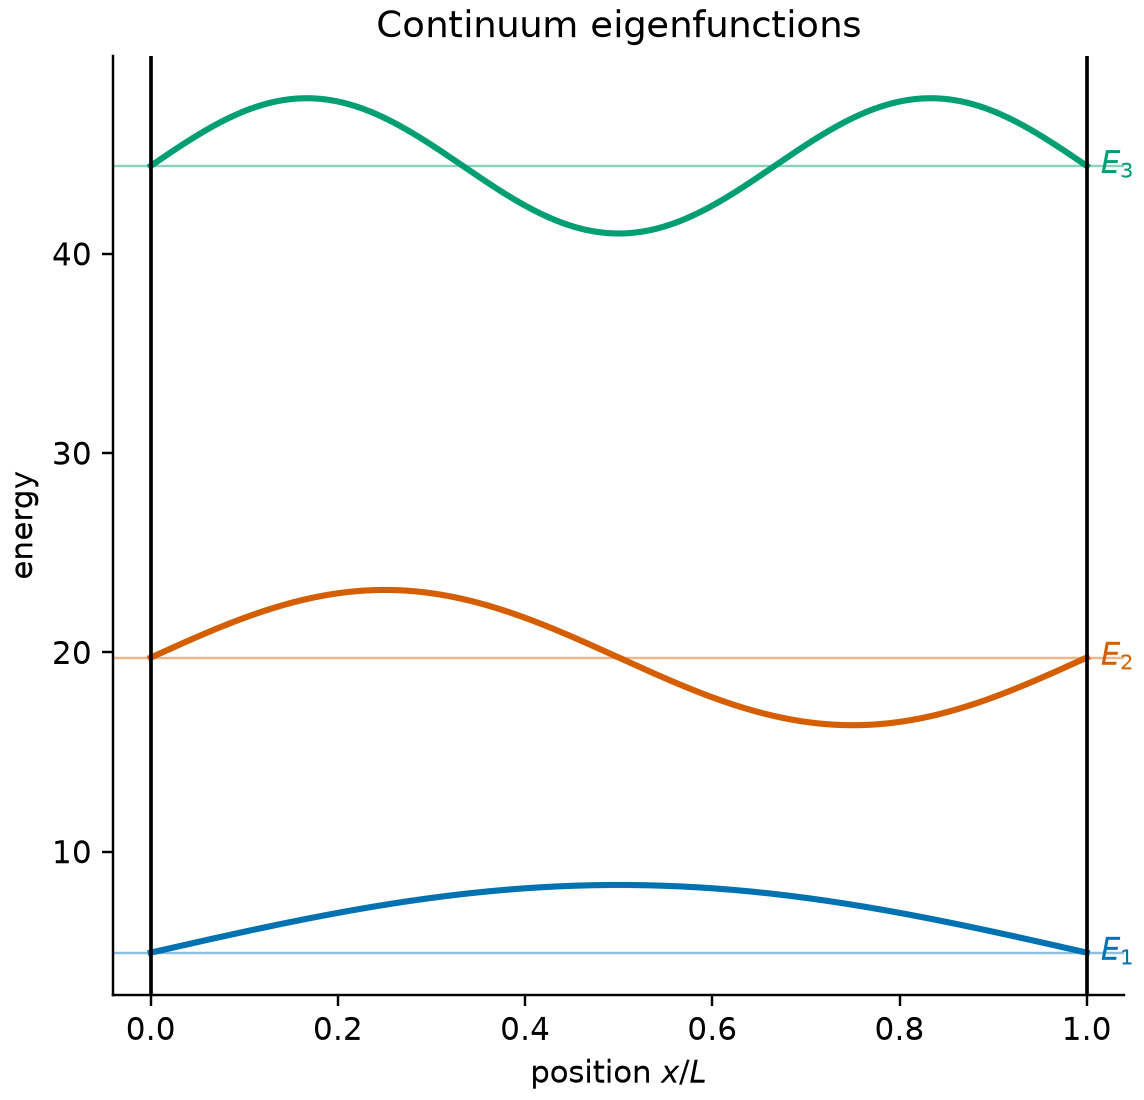
\includegraphics[width=\linewidth]{figure_01a_continuum_wavefunction_ladder.png}
 \caption{Continuum eigenfunctions centered on $E_n$.}
 \label{fig:wavefunction-ladders-continuum}
\end{subfigure}\hfill
\begin{subfigure}[t]{0.48\linewidth}
 \centering
 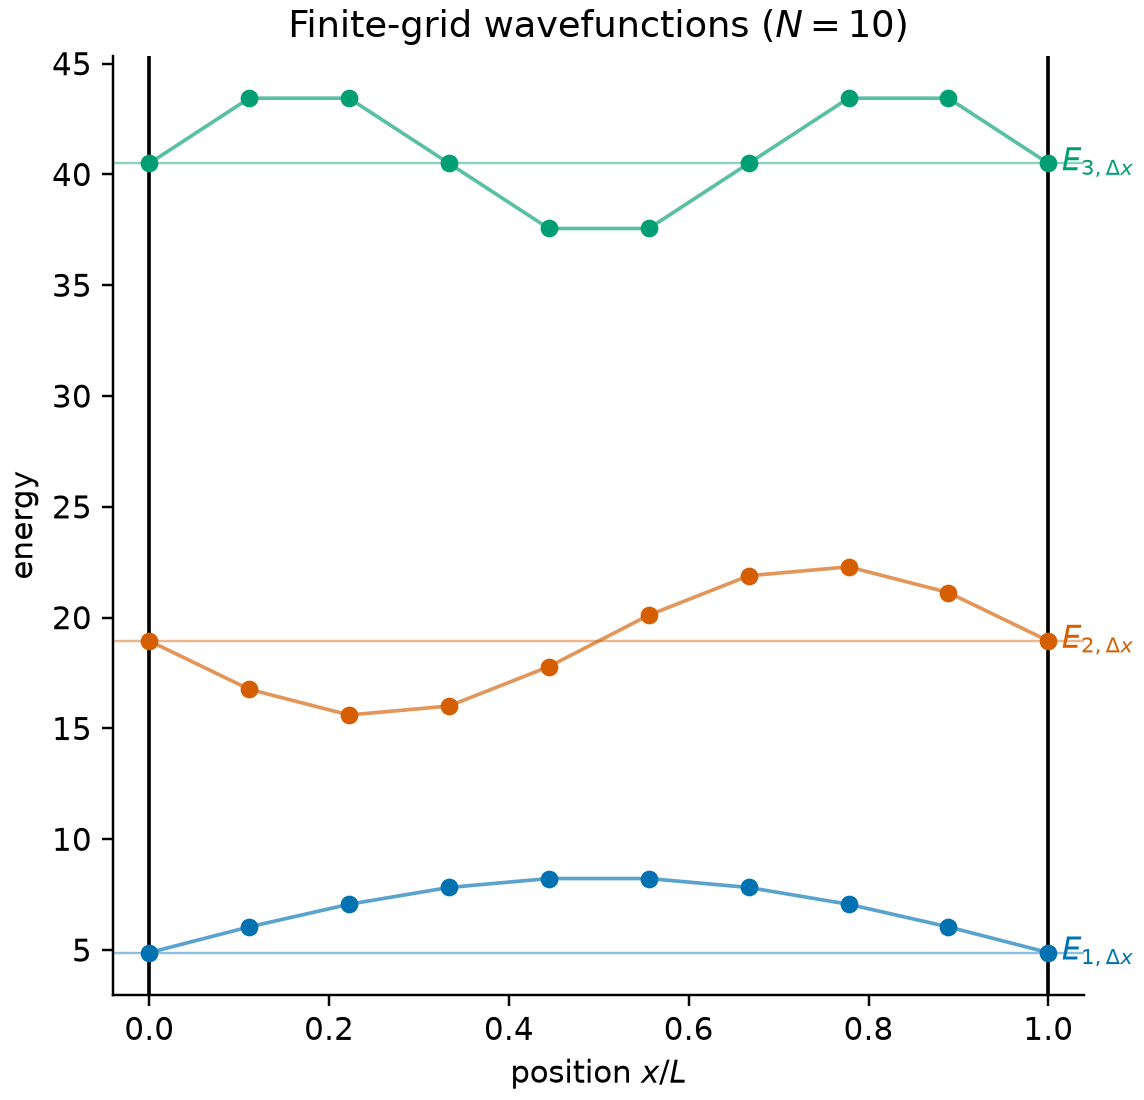
\includegraphics[width=\linewidth]{figure_01b_discrete_wavefunction_ladder.png}
 \caption{Finite-grid wavefunctions centered on $E_{n,\Delta x}$.}
 \label{fig:wavefunction-ladders-discrete}
\end{subfigure}
\caption{The first three PIAB1D states shown as energy ladders. The vertical
wavefunction displacement is scaled for visibility; the horizontal reference line in
each trace marks its associated energy.}
\label{fig:wavefunction-ladders}
\end{figure}

Equation~\eqref{eq:finite-hamiltonian} is the usual centered approximation to
Equation~\eqref{eq:continuum-operator} \cite{strikwerda2004}. The spectra in
Equations~\eqref{eq:continuum-spectrum} and \eqref{eq:discrete-spectrum} are exact
solutions of different eigenvalue problems.

\FloatBarrier
\subsection{Spectral reconstruction}

On the mathematical side, the spectral theorem reconstructs a self-adjoint operator
$H$ from its projection-valued measure $P_H$ \cite{reedSimon1980,teschl2014}:
\begin{equation}
 I=\int_{\RR}\mathrm{d}P_H(\lambda),
 \qquad
 H=\int_{\RR}\lambda\,\mathrm{d}P_H(\lambda).
 \label{eq:general-spectral-construction}
\end{equation}
The second integral is interpreted on the operator domain of $H$. In the physics
formulation, an observable $A$ with a pure-point spectrum has the spectral
reconstruction
\begin{equation}
 I=\sum_a P_a,
 \qquad
 A=\sum_a aP_a,
 \label{eq:physics-operator-reconstruction}
\end{equation}
where $P_a$ projects onto the eigenspace with measured value $a$. For a
nondegenerate spectrum, $P_a=\lvert a\rangle\langle a\rvert$. This is the standard
operator construction from eigenvalues and eigenstates used by Shankar and by
Sakurai and Napolitano \cite{shankar1994,sakuraiNapolitano2020}. Specializing it to
the box gives
\begin{equation}
 I=\sum_{n=1}^{\infty}
 \lvert\psi_n\rangle\langle\psi_n\rvert,
 \qquad
 H_{\mathrm{box}}=\sum_{n=1}^{\infty}
 E_n\lvert\psi_n\rangle\langle\psi_n\rvert.
 \label{eq:continuum-spectral-construction}
\end{equation}
The second equality is understood through the action of the spectral series on states
in $\mathcal D(H_{\mathrm{box}})$. The finite matrix has the corresponding complete
spectral reconstruction \cite{hornJohnson2013,golubVanLoan2013}:
\begin{equation}
 \mat{H}_{\Delta x}
 =\sum_{n=1}^{N-2}E_{n,\Delta x}
 \vect{\psi}_{n,\Delta x}\vect{\psi}_{n,\Delta x}^{\mathsf T}.
 \label{eq:finite-spectral-construction}
\end{equation}

\subsection{Operator reduction}

The time-independent Schr\"odinger equation identifies the energy eigenstates and
their energies:
\begin{equation}
 H_{\mathrm{box}}\lvert\psi_n\rangle
 =E_n\lvert\psi_n\rangle.
 \label{eq:tise-spectral-eigenpair}
\end{equation}
A state in the operator domain can be expanded in the complete energy basis as
\begin{equation}
 \lvert\psi\rangle=\sum_{n=1}^{\infty}c_n\lvert\psi_n\rangle,
 \qquad
 c_n=\langle\psi_n\vert\psi\rangle.
 \label{eq:state-spectral-expansion}
\end{equation}
Applying the Hamiltonian gives
\begin{equation}
 H_{\mathrm{box}}\lvert\psi\rangle
 =\sum_{n=1}^{\infty}E_n c_n\lvert\psi_n\rangle.
 \label{eq:hamiltonian-spectral-action}
\end{equation}
This componentwise action is the physics form of the spectral reconstruction
\cite{shankar1994,sakuraiNapolitano2020}. Thus $E_n$ is the spectral multiplier that scales the $n$th component under the
action of the Hamiltonian. The coefficient $c_n$ is the state's expansion amplitude,
and $\lvert c_n\rvert^2$ is its measurement probability when the state is normalized;
the magnitude of $E_n$ is not itself a probability weight. Energy eigenvalues enter
probability assignments only after a statistical ensemble has been specified. In the
canonical ensemble, the equilibrium probability of the nondegenerate energy state
$n$ is
\begin{equation}
 p_n=\frac{\exp(-\beta E_n)}{Z},
 \qquad
 Z=\sum_j\exp(-\beta E_j),
 \qquad
 \beta=\frac{1}{k_{\mathrm B}T},
 \label{eq:canonical-boltzmann-probability}
\end{equation}
as described by Pathria and Beale \cite{pathriaBeale2011}. These Boltzmann
probabilities depend on the chosen ensemble and temperature and are distinct from the
Born probabilities $\lvert c_n\rvert^2$ of a specified pure state.

We use this interpretation to motivate basis truncation in the Hamiltonian reduction.
For a pure state, the probability omitted above mode $M$ is
$\sum_{n>M}\lvert c_n\rvert^2$. For a canonical ensemble, the corresponding omitted
thermal probability is
\begin{equation}
 w_{>M}^{(\beta)}
 =\frac{1}{Z}\sum_{n>M}\exp(-\beta E_n).
 \label{eq:omitted-canonical-weight}
\end{equation}
A low-energy truncation is therefore appropriate when the intended states have little
amplitude outside the retained subspace or when the omitted thermal weight is small at
the temperature of interest.

A reduction selects a spectral subset and restricts the operator to its span. For the
lowest $M$ box states, define
\begin{equation}
 P_M=\sum_{n=1}^{M}\lvert\psi_n\rangle\langle\psi_n\rvert,
 \qquad
 H^{(M)}=P_MH_{\mathrm{box}}P_M
 =\sum_{n=1}^{M}E_n\lvert\psi_n\rangle\langle\psi_n\rvert.
 \label{eq:continuum-operator-reduction}
\end{equation}
The finite calculation applies the same construction to the complete matrix spectrum.
Let
$\mat{U}_M=[\vect{\psi}_{1,\Delta x}\ \cdots\ \vect{\psi}_{M,\Delta x}]
\in\RR^{(N-2)\times M}$ contain the lowest $M$ normalized represented wavefunctions
of $\mat{H}_{\Delta x}$. The spectral projector, its
complement, and the reduced Hamiltonian are
\begin{equation}
 \mat{P}_M=\mat{U}_M\mat{U}_M^{\mathsf T},\qquad
 \mat{Q}_M=\mat{I}_{N-2}-\mat{P}_M,\qquad
 \mat{H}_{\mathrm{red}}
 =\mat{U}_M^{\mathsf T}\mat{H}_{\Delta x}\mat{U}_M.
 \label{eq:reduction-definitions}
\end{equation}
Define the diagonal matrix
\begin{equation}
 \mat{D}_{\Delta x}
 =\operatorname{diag}(E_{1,\Delta x},\ldots,E_{M,\Delta x}).
\end{equation}
Because the columns of $\mat{U}_M$ are represented eigenfunctions,
\begin{equation}
 \mat{H}_{\Delta x}\mat{U}_M=\mat{U}_M\mat{D}_{\Delta x},\qquad
 \mat{H}_{\mathrm{red}}=\mat{D}_{\Delta x},\qquad
 \mat{Q}_M\mat{H}_{\Delta x}\mat{U}_M=\mat{0}.
 \label{eq:exact-reduction}
\end{equation}
These are finite-dimensional spectral identities
\cite{hornJohnson2013,golubVanLoan2013}. The last equality states that the selected
finite eigenspace has no leakage into its orthogonal complement.

The embedded operator $\mat{P}_M\mat{H}_{\Delta x}\mat{P}_M$ is an
$(N-2)\times(N-2)$ matrix. The coordinate matrix $\mat{H}_{\mathrm{red}}$ is an $M\times M$ matrix. They describe
the same restriction in different representations, but they cannot be subtracted
without an explicit map between those representations.

A similar distinction separates the discrete and continuum spectral references. Set
\begin{equation}
 \mat{D}=\operatorname{diag}(E_1,\ldots,E_M).
\end{equation}
Then
\begin{equation}
 \mat{H}_{\Delta x}\mat{U}_M
 -\mat{U}_M\mat{D}_{\Delta x}=\mat{0},
 \label{eq:discrete-reference-residual}
\end{equation}
whereas
\begin{equation}
 \mat{H}_{\Delta x}\mat{U}_M-\mat{U}_M\mat{D}
 =\mat{U}_M(\mat{D}_{\Delta x}-\mat{D}).
 \label{eq:continuum-reference-residual}
\end{equation}
The second residual measures finite-difference dispersion. It is not a failure of the
projection.

The retained dimension $M$ is therefore an explicit resolution parameter of the
operator reduction. We now describe a diagnostic methodology for choosing $M$. The
method compares candidate retained subspaces through omitted spectral weight,
retained-mode dispersion, spectral leakage, and operator-residual norms, then applies
a declared selection rule to the admissible candidates.

\section{Methodology}

Because PIAB1D has both an analytical continuum solution and an exact discrete
representation, it provides a clean sandbox for studying operator reduction by
spectral reduction. The calculation separates diagnostics of the eigensolver, the
finite-difference approximation, the spectral projection, and the interpretation of
operator residuals.

\subsection{Calculation design}

All calculations use the nondimensional convention $L=m=\hbar=1$. The core
calculation uses $N=10$ points on the closed interval, hence eight interior degrees of
freedom. The canonical-weight calculation in Section~4.1 selects the lowest $M=3$
represented energy--wavefunction pairs. The grid studies evaluate every closed-interval grid size
\begin{equation}
 N=10,11,\ldots,258,
 \label{eq:grid-series}
\end{equation}
which corresponds to every interior dimension $N-2=8,9,\ldots,256$. The
eigensystems are computed in binary64 arithmetic by the pinned PhysKit PIAB1D
finite-difference solver. Quadrature handling is enabled explicitly in the retained
input. The result stores the Euclidean-normalized solver vectors separately from the
quadrature-normalized nodal amplitudes, together with the endpoint-inclusive
trapezoidal-rule identity, spacing, full and interior weights, and diagonal mass
matrix. The unit-free rule and its homogeneous-Dirichlet restriction are supplied by
Project Koios Numerics, while PhysKit applies the weights to the sampled quantum
states. Because the present interior quadrature matrix is a scalar multiple of the
identity, Equation~\eqref{eq:quadrature-invariance} shows that this rescaling leaves
every projector, reduced matrix, and residual reported here unchanged. The
Hamiltonian is still solved as a standard real-symmetric eigenproblem, not as a
generalized-mass-matrix eigenproblem. A nonuniform grid, nonconstant rule, or
consistent finite-element mass matrix is outside the present calculation.

Separate verification scripts recompute the closed discrete spectrum, spectral
reconstruction, projector identities, retained embeddings, and residual formulas.

\subsection{Implemented reduction representations}

For the core calculation, define
$\boldsymbol{\Phi}_M:=\mat{U}_M\in\RR^{8\times3}$. This reduction basis is distinct
from the complementary projector $\mat{Q}_M=\mat{I}_{N-2}-\mat{P}_M$ in
Equation~\eqref{eq:reduction-definitions}. The implementation binds the aligned
representations in one \texttt{ReducedHamiltonian} object:
\begin{description}
 \item[\texttt{spectral\_subspace}] An
 \texttt{OrthogonalSpectralSubspace} whose \texttt{basis\_vectors} are
 $\boldsymbol{\Phi}_M$, an $8\times3$ matrix whose columns are the three selected
 eigenvectors. Its \texttt{projector()} method derives
 $\mat{P}_M=\boldsymbol{\Phi}_M\boldsymbol{\Phi}_M^{\mathsf T}$, the $8\times8$
 orthogonal projector onto the selected subspace.
 \item[\texttt{matrix}]
 $\boldsymbol{\Phi}_M^{\mathsf T}\mat{H}_{\Delta x}\boldsymbol{\Phi}_M$,
 the $3\times3$ reduced Hamiltonian used by the decomposition.
 \item[\texttt{embedded.matrix}]
 $\boldsymbol{\Phi}_M
 (\boldsymbol{\Phi}_M^{\mathsf T}\mat{H}_{\Delta x}\boldsymbol{\Phi}_M)
 \boldsymbol{\Phi}_M^{\mathsf T}$, the $8\times8$ reduced Hamiltonian mapped back
 onto the full grid space.
\end{description}
The abstract \texttt{SpectralSubspace} contract does not assert that every Hamiltonian
has an orthogonal spectral projector. PIAB1D uses the concrete orthogonal case because
its represented Hamiltonian is real symmetric. The reduced and embedded matrices
represent the same restricted operator on different coordinate spaces. The projector
records which full-space states belong to that reduction; the complementary projector
remains $\mat{Q}_M=\mat{I}_{N-2}-\mat{P}_M$.

Three numerical questions are considered. The first is whether the computed finite
matrix agrees with the exact discrete formulas. The second is how fixed and growing
mode indices behave as the grid is refined. The third is how the meaning of a
residual changes when compression, boundary closure, norm, or admissible model class
changes.

\subsection{Spectral and reduction diagnostics}

\subsubsection{Computed energy--wavefunction inventory}

Let $(\widetilde E_{n,\Delta x},
\widetilde{\vect{\psi}}_{n,\Delta x})$ denote the computed represented eigenpair,
ordered by increasing energy. Collect the complete computed wavefunction basis and
its energies as
\begin{equation}
 \mat{U}=[\widetilde{\vect{\psi}}_{1,\Delta x}\ \cdots\
 \ \widetilde{\vect{\psi}}_{N-2,\Delta x}],
 \qquad
 \widetilde{\mat{D}}_{\Delta x}
 =\operatorname{diag}(\widetilde E_{1,\Delta x},\ldots,
 \widetilde E_{N-2,\Delta x}).
 \label{eq:computed-eigenpair-inventory}
\end{equation}
Thus $\mat{U}\in\RR^{(N-2)\times(N-2)}$ contains every computed represented
wavefunction, while $\widetilde{\mat{D}}_{\Delta x}$ contains the corresponding
computed energies.
All matrix residuals below use the Frobenius norm
\begin{equation}
 \lVert\mat{A}\rVert_{\fro}
 =\left(\sum_{i,j}\lvert A_{ij}\rvert^2\right)^{1/2}.
 \label{eq:frobenius-norm}
\end{equation}
It aggregates every matrix-entry discrepancy into one nonnegative scalar.

\subsubsection{Closed-form discrete-spectrum agreement}

The discrete-spectrum diagnostic is
\begin{equation}
 \delta_E
 =\max_{1\leq n\leq N-2}
 \left\lvert\widetilde E_{n,\Delta x}
 -E_{n,\Delta x}\right\rvert.
 \label{eq:discrete-spectrum-diagnostic}
\end{equation}
For each mode, the calculation subtracts the exact represented energy in
Equation~\eqref{eq:discrete-spectrum} from the corresponding computed energy, takes
the absolute value, and reports the largest discrepancy. This tests whether the
eigensolver and the assembled finite matrix reproduce the known spectrum of the
discrete problem. It does not compare the discrete spectrum with the continuum
energies $E_n$.

\subsubsection{Full spectral reconstruction}

The complete computed eigensystem is used to reconstruct the represented Hamiltonian,
and the discrepancy is measured by
\begin{equation}
 \delta_{\mathrm{rec}}
 =\left\lVert\mat{H}_{\Delta x}
 -\mat{U}\widetilde{\mat{D}}_{\Delta x}\mat{U}^{\mathsf T}\right\rVert_{\fro}.
 \label{eq:spectral-reconstruction-diagnostic}
\end{equation}
The calculation forms the matrix product
$\mat{U}\widetilde{\mat{D}}_{\Delta x}\mat{U}^{\mathsf T}$, subtracts it from the
assembled Hamiltonian, and evaluates the Frobenius norm of the difference. A small
$\delta_{\mathrm{rec}}$ checks the completeness and mutual consistency of the computed
energies and represented wavefunctions. It also detects mismatched
energy--wavefunction ordering. It does not establish that $\mat{H}_{\Delta x}$ accurately represents the
continuum operator.

\subsubsection{Projector idempotency}

The retained represented wavefunctions define
$\mat{P}_M=\mat{U}_M\mat{U}_M^{\mathsf T}$. Its
idempotency defect is
\begin{equation}
 \delta_{\mathrm{idem}}
 =\lVert\mat{P}_M^2-\mat{P}_M\rVert_{\fro}.
 \label{eq:projector-idempotency-diagnostic}
\end{equation}
The calculation applies the projector twice, subtracts one application, and measures
the remaining matrix. An exact projector satisfies $\mat{P}_M^2=\mat{P}_M$, so this
diagnostic checks that the computed retained basis produces a numerically valid
projection.

\subsubsection{Retained coordinate representation}

The reduced coordinate matrix should equal the diagonal matrix of the selected exact
discrete eigenvalues. The diagnostic is
\begin{equation}
 \delta_{\mathrm{coord}}
 =\lVert\mat{H}_{\mathrm{red}}-\mat{D}_{\Delta x}\rVert_{\fro}.
 \label{eq:retained-coordinate-diagnostic}
\end{equation}
Here the calculation constructs
$\mat{H}_{\mathrm{red}}=\mat{U}_M^{\mathsf T}
\mat{H}_{\Delta x}\mat{U}_M$, subtracts
$\mat{D}_{\Delta x}=\operatorname{diag}(E_{1,\Delta x},\ldots,
E_{M,\Delta x})$, and measures the difference. A small value confirms that the
retained basis diagonalizes the represented Hamiltonian with the expected discrete
energies.

\subsubsection{Retained embedding}

The same reduced operator can be represented either directly in the full coordinate
space or lifted from retained coordinates. Their discrepancy is
\begin{equation}
 \delta_{\mathrm{embed}}
 =\left\lVert\mat{P}_M\mat{H}_{\Delta x}\mat{P}_M
 -\mat{U}_M\mat{H}_{\mathrm{red}}\mat{U}_M^{\mathsf T}\right\rVert_{\fro}.
 \label{eq:retained-embedding-diagnostic}
\end{equation}
The first term compresses the Hamiltonian in the full $(N-2)$-dimensional coordinate
space. The second term maps the $M\times M$ reduced coordinate matrix back into that
space. This diagnostic is important because matrices of different dimensions cannot
be compared until an explicit embedding has placed them in the same representation.

\subsubsection{Spectral leakage}

The leakage diagnostic is
\begin{equation}
 \delta_{\mathrm{leak}}
 =\lVert\mat{Q}_M\mat{H}_{\Delta x}\mat{U}_M\rVert_{\fro}.
 \label{eq:spectral-leakage-diagnostic}
\end{equation}
The product $\mat{H}_{\Delta x}\mat{U}_M$ applies the Hamiltonian to every retained
basis vector, and left multiplication by $\mat{Q}_M$ extracts the component outside
the retained subspace. A zero value means that the subspace is invariant under the
represented Hamiltonian. This vanishes analytically for a subspace spanned by exact represented
wavefunctions; it need not vanish for a general trial subspace.

Together these diagnostics test distinct finite-dimensional identities. None of them
measures error with respect to the continuum operator; that comparison requires the
dispersion diagnostics introduced next.

\subsection{Continuum-dispersion diagnostics}

The relative energy error of mode $n$ is
\begin{equation}
 \epsilon_{n,N}
 =\frac{\left\lvert\widetilde E_{n,\Delta x}-E_n\right\rvert}{E_n}.
 \label{eq:relative-energy-error}
\end{equation}
For two successive grids with spacings $\Delta x_k$ and $\Delta x_{k+1}$, the
observed order is
\begin{equation}
 p_{n,k}
 =\frac{\log(\epsilon_{n,k}/\epsilon_{n,k+1})}
 {\log(\Delta x_k/\Delta x_{k+1})}.
 \label{eq:observed-order}
\end{equation}
Fixed-$n$ sequences test pointwise spectral convergence. Sequences with
$q=n/(N-1)$ approximately fixed test modes whose index grows with the grid. These are
different convergence questions. Such high-frequency nonuniformity is a known feature
of finite-difference wave models \cite{zuazua2005}; the exact PIAB1D spectrum lets us
exhibit it directly for a stationary eigenvalue problem.

\subsection{Operator-residual and model-class diagnostics}

Residual-based a posteriori estimators can relate a reduced-model residual to an error
when the governing problem supplies the necessary stability assumptions and constants
\cite{fengChellappaBenner2024}. The residuals here have a different purpose: they
distinguish which finite operators have been subtracted and are not asserted to be
general error bounds.

Three residual matrices are evaluated. Consistent compression compares the
Hamiltonian and kinetic matrix after applying the same projector,
\begin{equation}
 \mat{R}_{\mathrm{cons}}
 =\mat{P}_M\mat{H}_{\Delta x}\mat{P}_M
 -\mat{P}_M\mat{T}_{\mathrm{D},\Delta x}\mat{P}_M.
 \label{eq:method-consistent-residual}
\end{equation}
Unmatched compression compares the embedded retained Hamiltonian with the uncompressed
kinetic matrix,
\begin{equation}
 \mat{R}_{\mathrm{un}}
 =\mat{P}_M\mat{H}_{\Delta x}\mat{P}_M
 -\mat{T}_{\mathrm{D},\Delta x},
 \label{eq:method-unmatched-residual}
\end{equation}
and the boundary-closure residual is
\begin{equation}
 \mat{R}_{\mathrm{bc}}
 =\mat{H}_{\mathrm{D},\Delta x}-\mat{H}_{\mathrm{cyclic},\Delta x}.
 \label{eq:method-boundary-residual}
\end{equation}
Each residual is measured with the Frobenius, spectral, and maximum-entry norms. The
same-grid normalized diagnostic is
\begin{equation}
 \eta_{*}(\mat{R})
 =\frac{\lVert\mat{R}\rVert_*}{\lVert\mat{H}_{\Delta x}\rVert_*},
 \qquad *\in\{\fro,2,\max\}.
 \label{eq:normalized-residual}
\end{equation}
These norms describe different matrix properties and are not interchangeable.

Hamiltonian identification usually asks whether unknown dynamical parameters can be
recovered from declared controls and measurements
\cite{leBrisEtAl2007,wangEtAl2020}. Operator inference instead learns reduced
operators from dynamical data, including under Hamiltonian structure
\cite{sharmaWangKramer2022,kramerPeherstorferWillcox2024}. The present question is
narrower and static: once a reduced real symmetric matrix is known, does that matrix
alone determine a unique additive decomposition within a declared pair of component
classes? To test this distinction, the fit of an illustrative shift $\mat{K}$ to an
admissible potential-matrix class $\mathcal C$ is summarized by
\begin{equation}
 \rho_{\mathcal C}(\mat{K})
 =\min_{\mat{V}\in\mathcal C}\lVert\mat{K}-\mat{V}\rVert_{\fro}.
 \label{eq:model-class-fit-diagnostic}
\end{equation}
A zero fit residual establishes membership in the declared matrix class; it does not
establish a physical interpretation.

\subsection{Diagnostic selection of the retained dimension}

The retained dimension $M$ is selected by requiring the reduced basis to retain a
prescribed fraction of a declared canonical ensemble. On the finite $N$-point representation,
define
\begin{equation}
 Z_{\Delta x}=\sum_{j=1}^{N-2}\exp(-\beta E_{j,\Delta x}),
 \qquad
 w_{>M}^{(\beta,\Delta x)}
 =\frac{1}{Z_{\Delta x}}
  \sum_{n=M+1}^{N-2}\exp(-\beta E_{n,\Delta x}).
 \label{eq:represented-omitted-canonical-weight}
\end{equation}
The omitted-probability tolerance $\tau$ is declared a priori, before any candidate
retained dimension is evaluated. The required retained dimension is then
\begin{equation}
 M_{\star}(N,\beta,\tau)
 =\min\left\{M\in\{1,\ldots,N-2\}:
 w_{>M}^{(\beta,\Delta x)}\leq\tau\right\}.
 \label{eq:retained-dimension-rule}
\end{equation}
The worked calculation declares the core grid $N=10$, inverse temperature $\beta=0.1$
in inverse nondimensional energy units, and tolerance $\tau=0.01$ before computing the
candidate weights. The calculation then returns the smallest low-energy basis that
retains at least $99\%$ of the declared canonical probability. The remaining diagnostics test the numerical and continuum
quality of the selected reduction.

\section{Results and discussion}

\subsection{An a priori tolerance selects a stable dimension}

Figure~\ref{fig:retained-dimension-selection} turns the selection rule into a decision
map. Because the retained dimension is discrete, $M_{\star}(\tau)$ consists of
horizontal plateaus separated by the canonical tail weights. The declared tolerance
$\tau=0.01$ lies inside the $M_{\star}=3$ plateau: one and two modes are insufficient,
whereas the third mode is the first to satisfy the requirement. Thus $M=3$ is an
output of the declared ensemble and tolerance, not a dimension chosen after inspecting
the subsequent residuals.

\begin{figure}[!htbp]
\centering
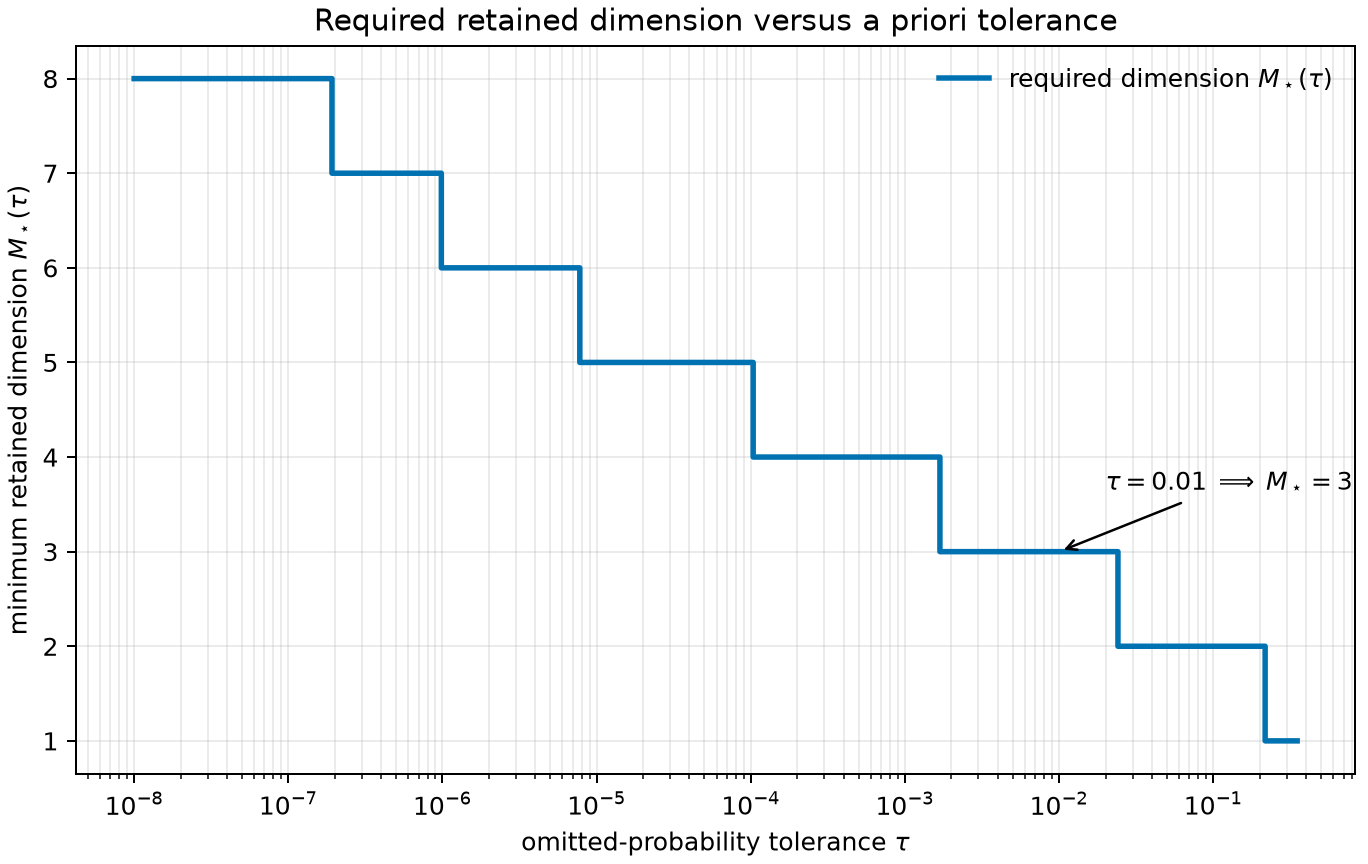
\includegraphics[width=0.86\linewidth]{figure_02_retained_dimension_selection.png}
\caption{Minimum retained dimension as a function of the a priori tolerance for
$N=10$ and $\beta=0.1$. Evaluating the step function at the declared value
$\tau=0.01$ gives $M_{\star}=3$.}
\label{fig:retained-dimension-selection}
\end{figure}

The plateau structure also makes the sensitivity of the decision visible. The selected
dimension changes only when the a priori tolerance crosses a canonical tail weight;
small tolerance perturbations within the same plateau leave the reduction unchanged.

\FloatBarrier

\subsection{Algebraic closure and continuum accuracy separate cleanly}

Figure~\ref{fig:finite-identity-diagnostics} reports every scalar diagnostic defined in
Section~3.2. The six curves remain in the binary64 roundoff regime throughout the grid
sweep, but they do not behave identically. Spectral reconstruction is the largest of
the full-space checks because it accumulates perturbations over an expanding matrix.
Within the retained sector, leakage grows most visibly with the finite-difference energy
scale, whereas the projector-idempotency defect remains essentially flat. This pattern
is the expected signature of unnormalized algebraic residuals: their absolute
magnitudes inherit representation scale even when the underlying identities continue
to close numerically.

\begin{figure}[!htbp]
\centering
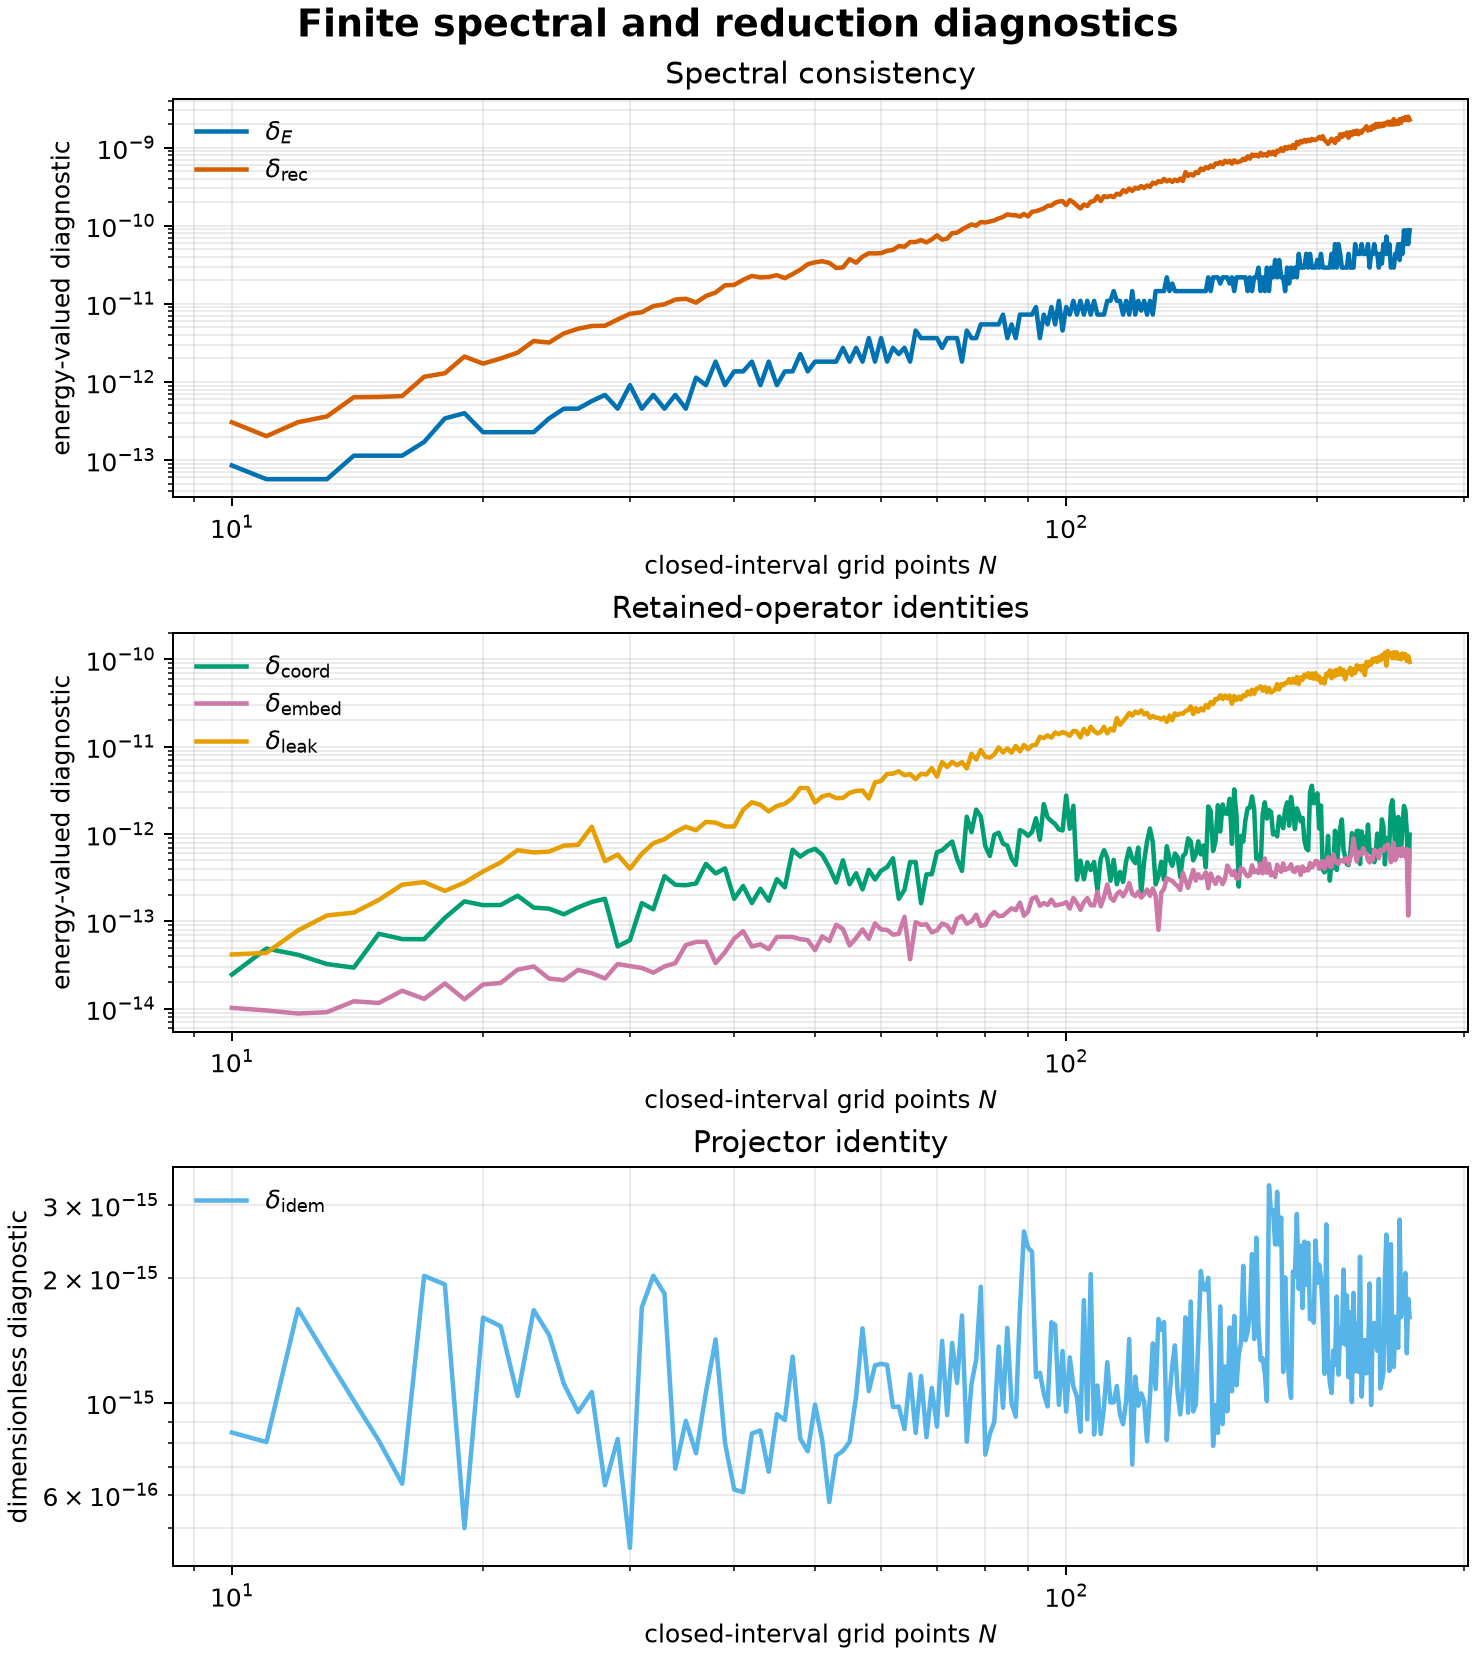
\includegraphics[width=0.82\linewidth]{finite-identity-diagnostics.png}
\caption{The six finite spectral and reduction diagnostics for every closed-interval
grid size $N=10,11,\ldots,258$, with retained dimension $M=3$. The curves correspond
directly to Equations~\eqref{eq:discrete-spectrum-diagnostic}--
\eqref{eq:spectral-leakage-diagnostic}. They test represented finite-dimensional
identities and do not measure continuum discretization error.}
\label{fig:finite-identity-diagnostics}
\end{figure}

The normalized eigensolver residuals in
Figure~\ref{fig:eigensolver-residual-norms} remove that representation scale. All three
norm ratios remain at roundoff, with no convergence curve to interpret. Their small
norm-dependent fluctuations show solver arithmetic rather than a physical or
continuum trend. Taken together, Figures~\ref{fig:finite-identity-diagnostics} and
\ref{fig:eigensolver-residual-norms} establish that the numerical eigensystem is
internally consistent before any comparison with the continuum model is made.

\begin{figure}[!htbp]
\centering
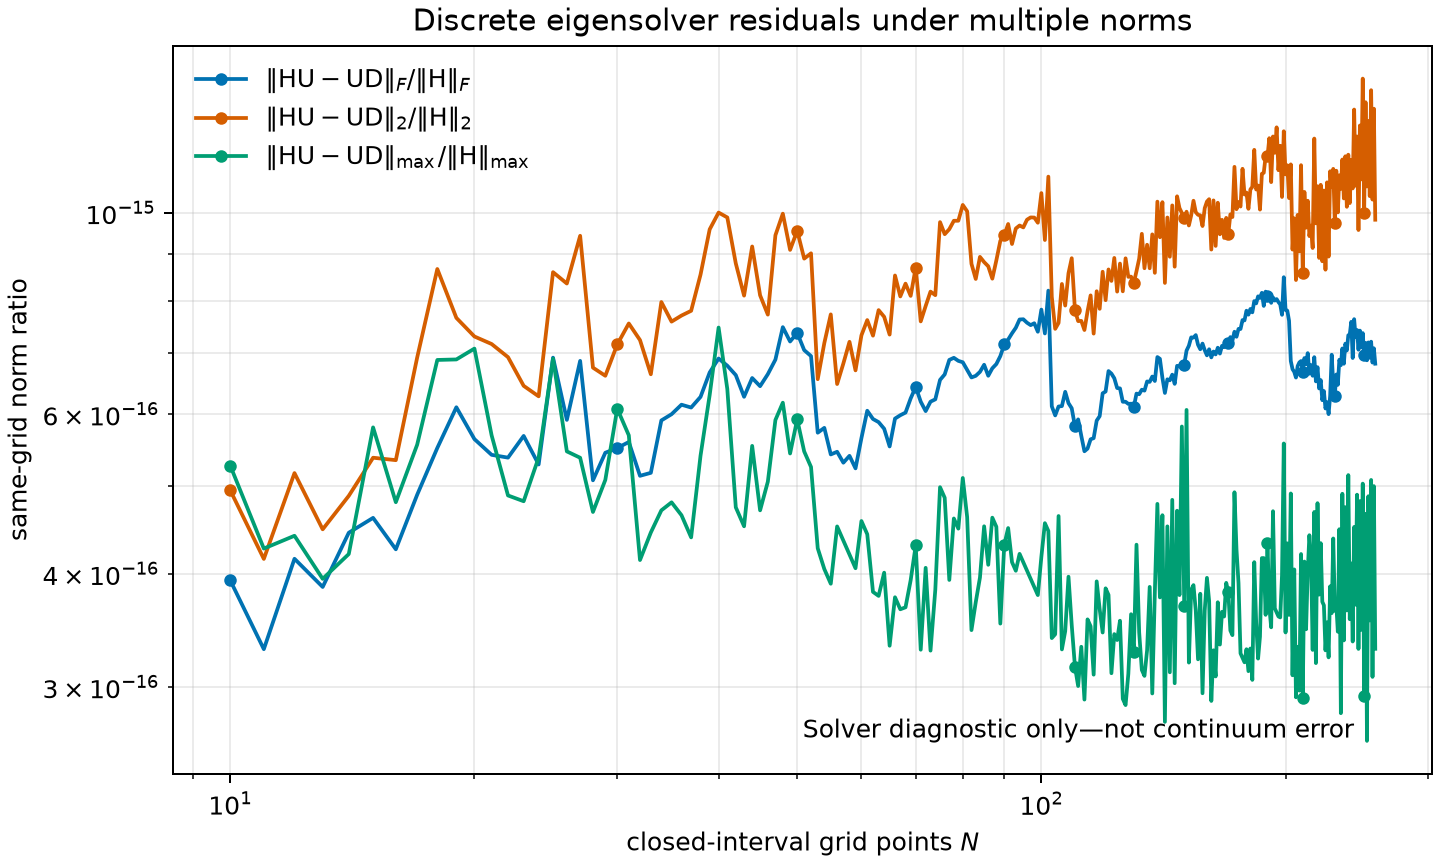
\includegraphics[width=0.94\linewidth]{eigensolver-residual-norms.png}
\caption{Full-eigensystem algebraic residuals under the Frobenius, spectral, and
maximum-entry norms. Matrices are shown in upright sans-serif notation in the figure.
The plotted quantities test $\mat{H}_{\Delta x}\mat{U}
-\mat{U}\widetilde{\mat{D}}_{\Delta x}$ and do not measure continuum error.}
\label{fig:eigensolver-residual-norms}
\end{figure}

Figure~\ref{fig:spectrum} then exposes a different phenomenon. The retained vectors
have the expected nodal sine structure, while the finite-difference energy ladder
bends progressively below the quadratic continuum ladder. The eigenvectors can
therefore be correct at the grid nodes even when their associated continuum energies
are biased. That separation between nodal geometry and energetic dispersion is the
central feature of this calibration problem.

\begin{figure}[ht]
\centering
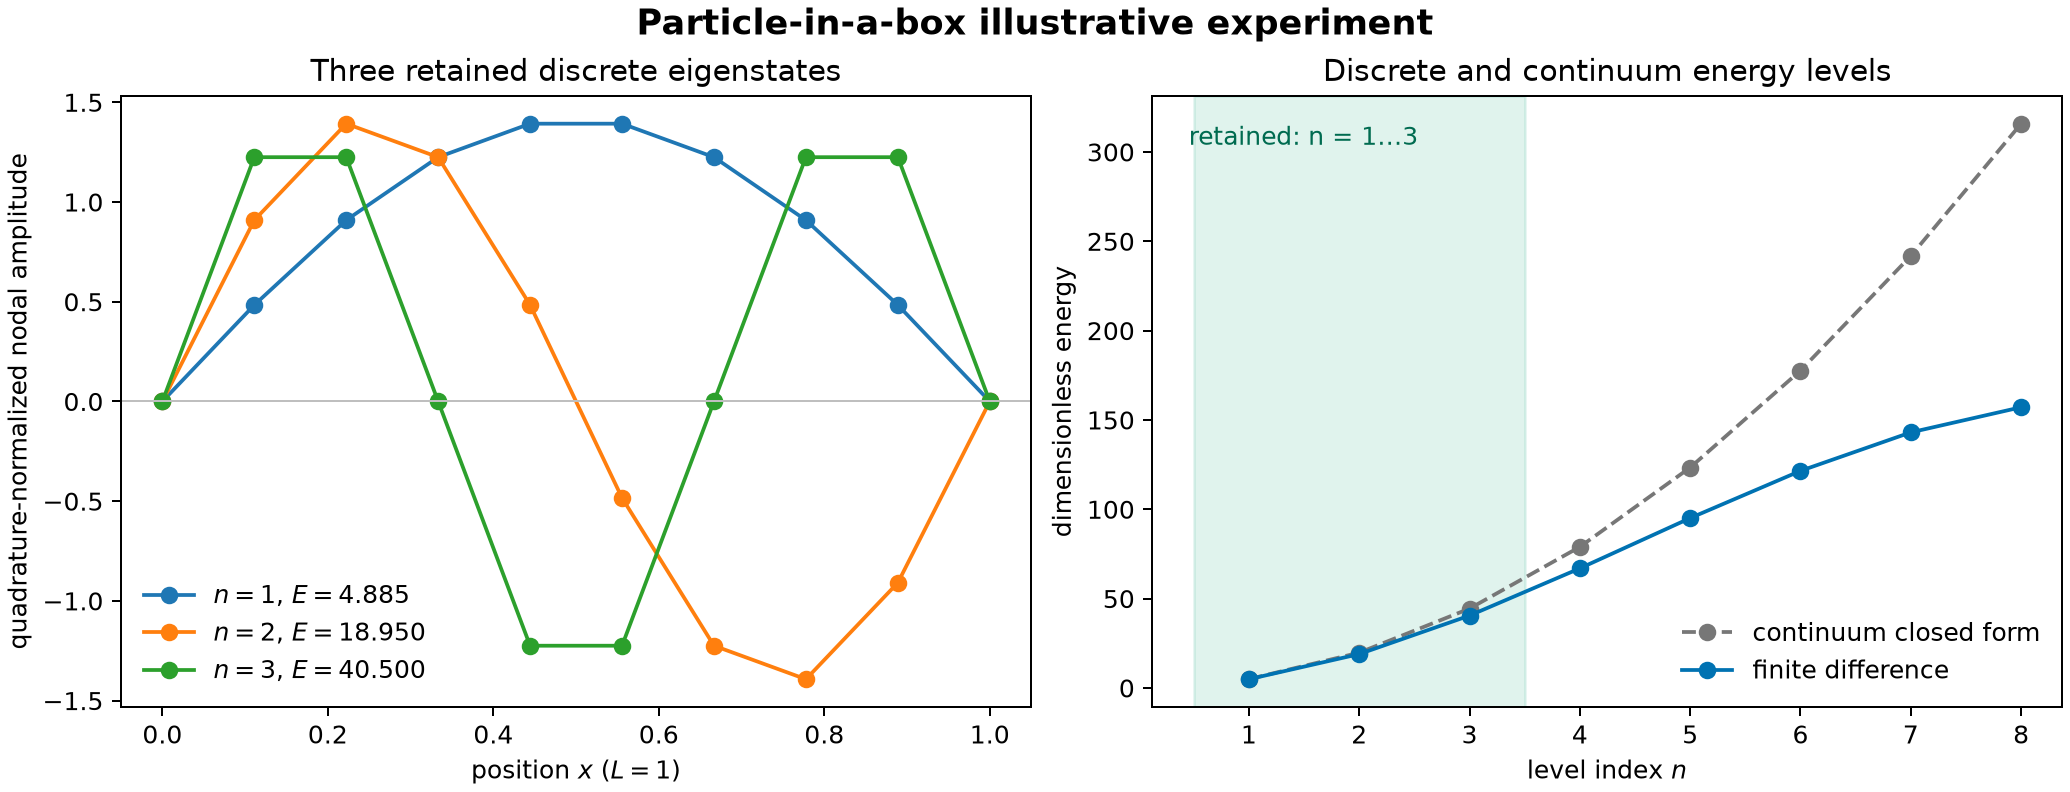
\includegraphics[width=\linewidth]{spectrum-and-states.png}
\caption{The three retained discrete eigenstates and the finite and continuum energy
levels for $N=10$ (eight interior points). Accurate solution of the discrete matrix does not remove its
finite-difference dispersion.}
\label{fig:spectrum}
\end{figure}

The mode-resolution map in Figure~\ref{fig:mode-resolution-sweep} makes the same
structure systematic. Every grid produces a rising error profile across mode index,
and refinement shifts the entire profile downward. Resolution is therefore controlled
by both $N$ and the wavelength being represented; a grid that is accurate for the
ground state need not be accurate for the upper part of even a small retained window.

\begin{figure}[!htbp]
\centering
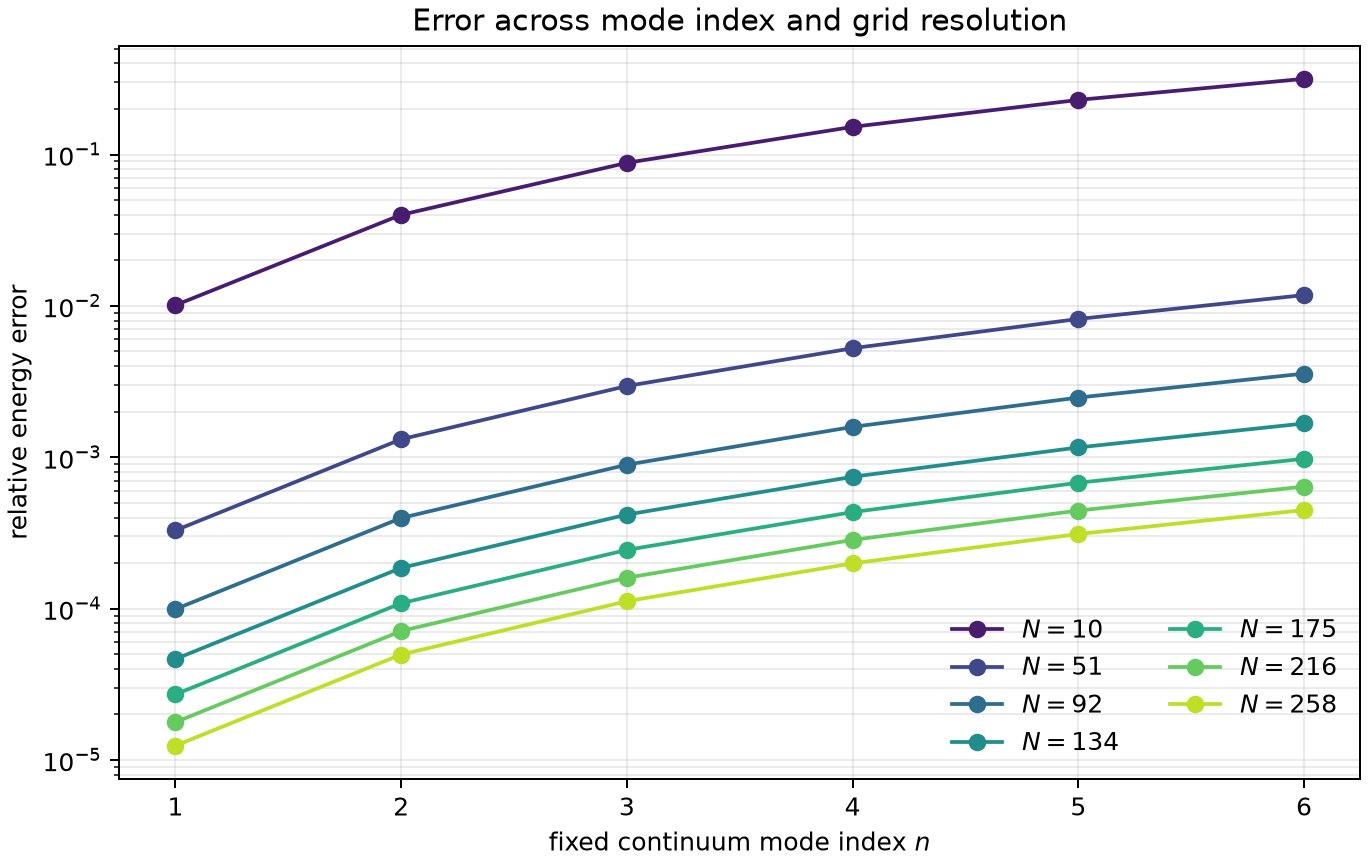
\includegraphics[width=0.82\linewidth]{convergence-mode-sweep.png}
\caption{Relative continuum-energy error across modes $n=1,\ldots,6$ for
representative closed-interval grids. The underlying calculation includes every
integer grid size from $N=10$ through $N=258$.}
\label{fig:mode-resolution-sweep}
\end{figure}

\FloatBarrier
\subsection{Convergence is modewise, not uniform over the spectrum}

The fixed low modes in Figure~\ref{fig:fixed-mode-convergence} follow parallel
second-order trajectories. Their observed orders approach two from below, while the
mode-dependent vertical offsets record the increasing dispersion penalty for shorter
wavelengths. Refinement therefore behaves exactly as the centered stencil predicts
when the mode index is held fixed.

\begin{figure}[ht]
\centering
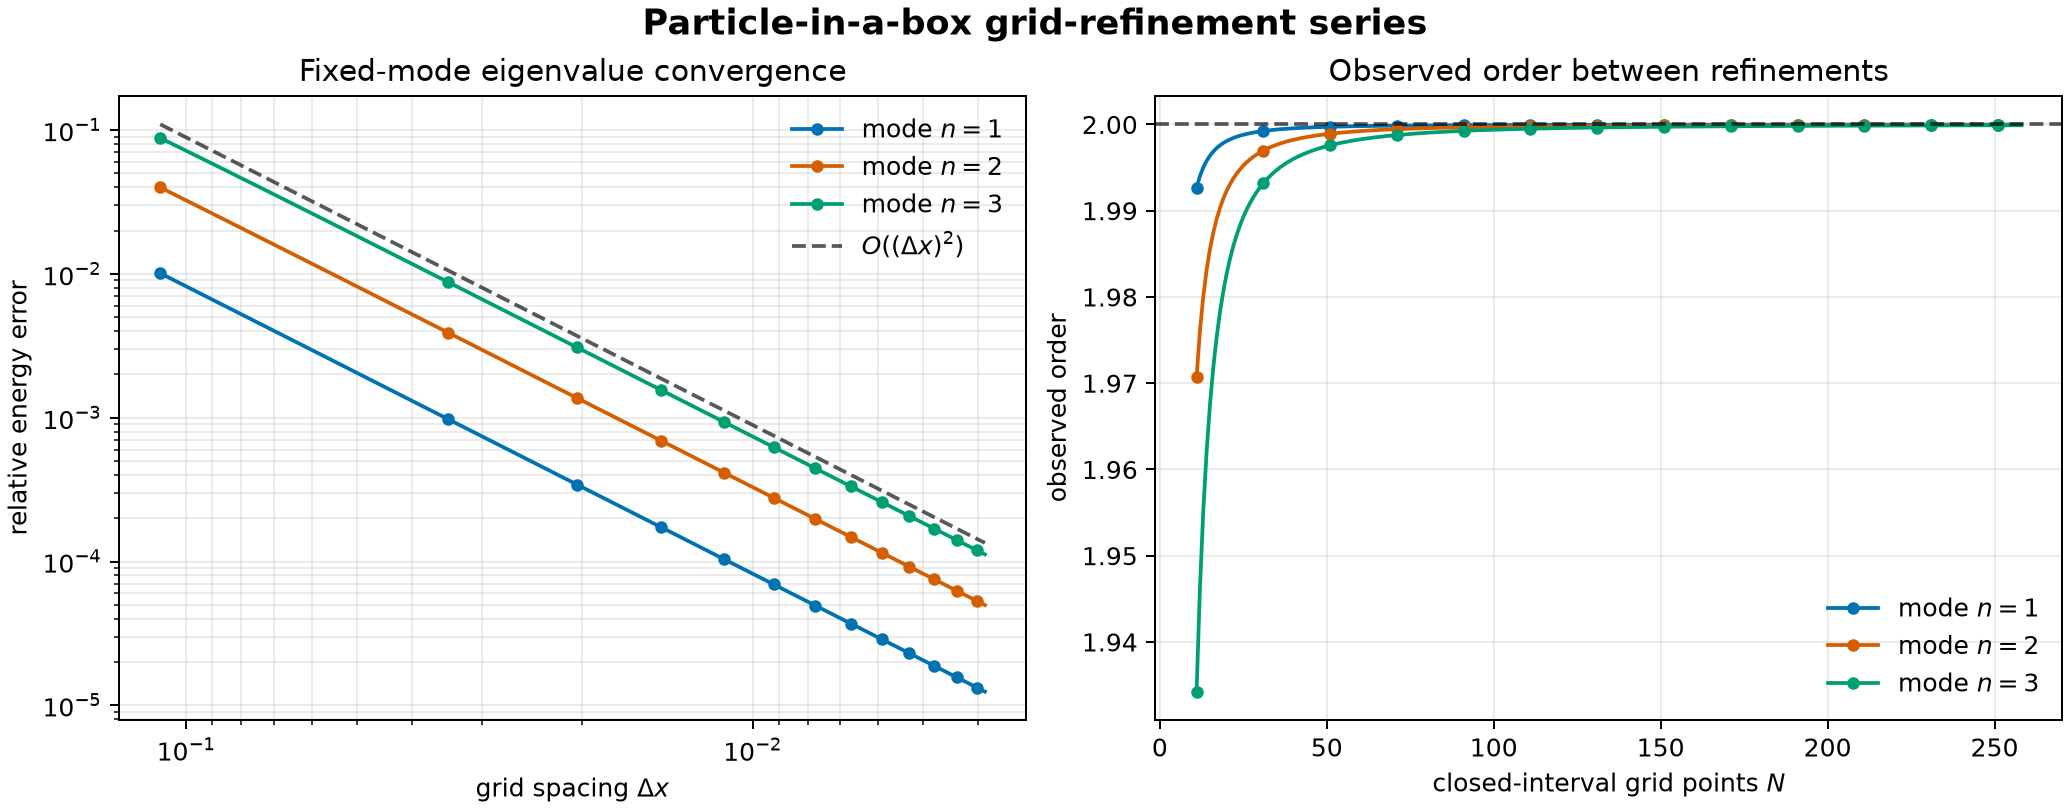
\includegraphics[width=0.94\linewidth]{convergence-series.png}
\caption{Relative energy error and observed refinement order for the first three
continuum modes. Each fixed mode approaches second-order convergence.}
\label{fig:fixed-mode-convergence}
\end{figure}

The conclusion changes when the mode index grows with the grid. In
Figure~\ref{fig:full-spectrum-sweep}, spectra from widely different matrix dimensions
collapse onto one dispersion curve when expressed in terms of the fractional index
$q=n/(N-1)$. Refinement adds higher-frequency modes but does not reduce the error at a
fixed nonzero $q$. Near the top of the spectrum the discrete energy remains far below
the continuum value, even though the nodal-overlap defects stay at roundoff. The plot
therefore separates two statements that a single residual cannot: the matrix
eigenproblem is solved accurately, but the stencil does not approximate all resolved
wavelengths uniformly.

\begin{figure}[!htbp]
\centering
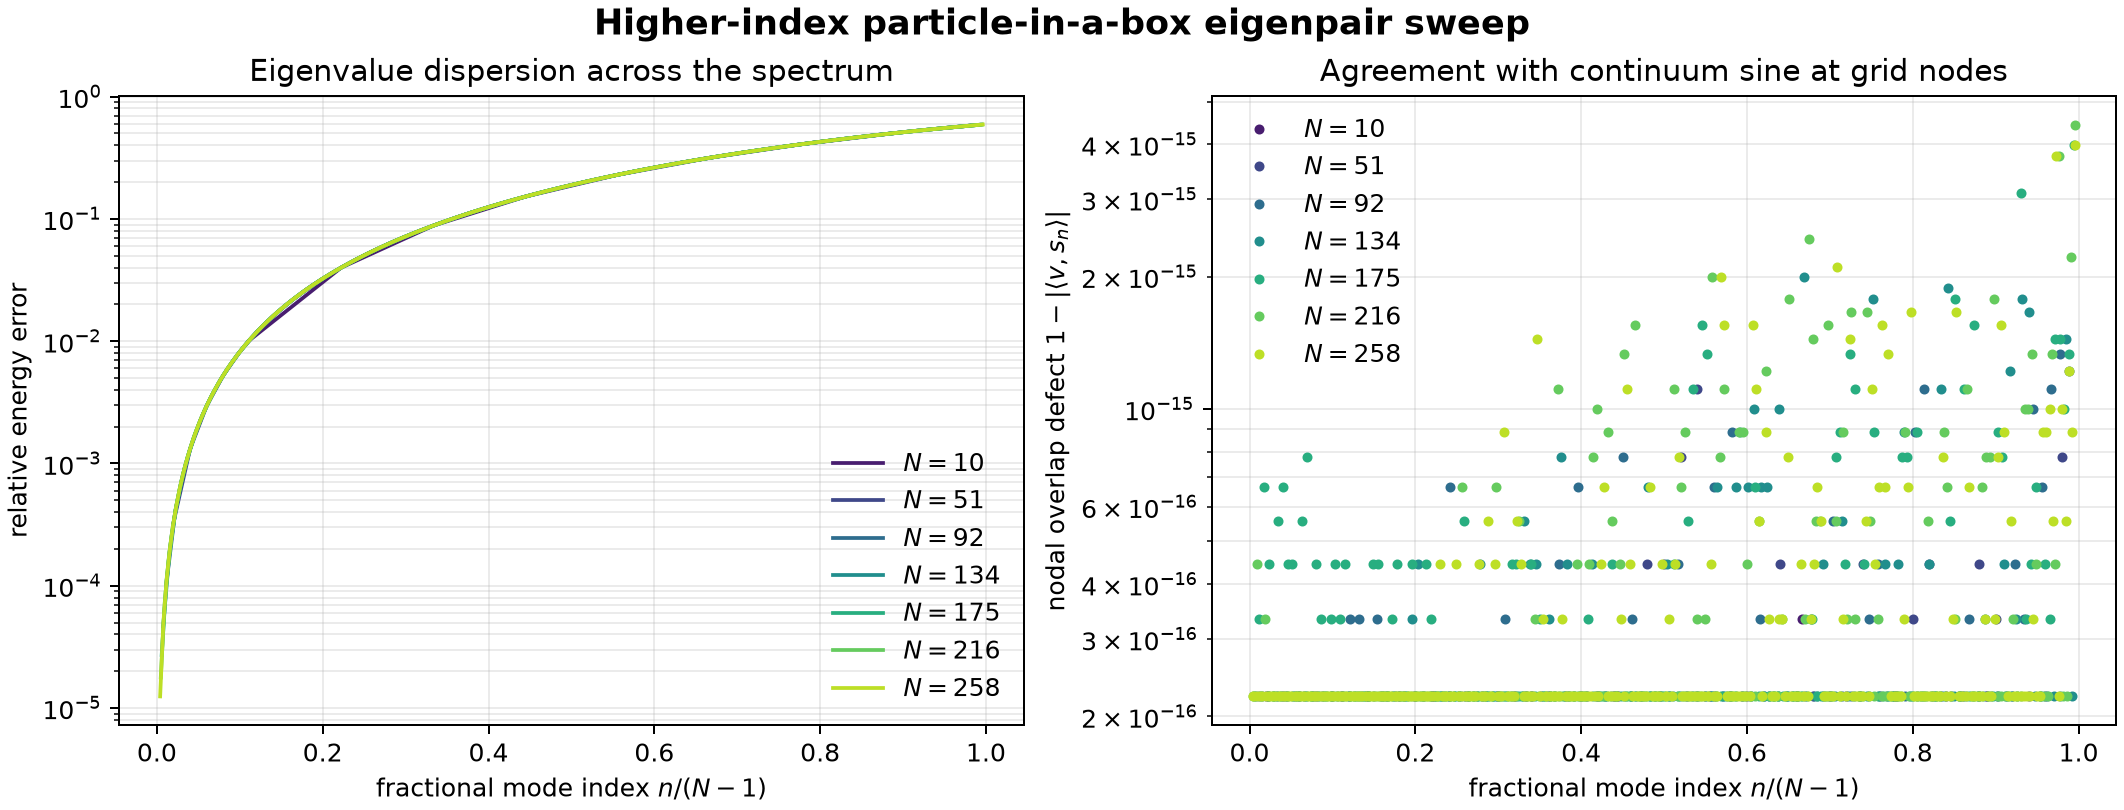
\includegraphics[width=\linewidth]{higher-eigenpair-sweep.png}
\caption{Full-spectrum diagnostics for representative members of the dense grid
sweep. The left panel shows finite-difference energy dispersion versus fractional
mode index. The right panel shows nodal wavefunction-overlap defects.}
\label{fig:full-spectrum-sweep}
\end{figure}

The higher fixed modes in Figure~\ref{fig:higher-mode-convergence} reconcile these two
views. Each eventually approaches second order, but the onset is delayed as the mode
index increases. Second-order convergence is thus an asymptotic statement about a
fixed physical mode, not a blanket statement about every eigenvalue returned by a
growing discretization.

\begin{figure}[ht]
\centering
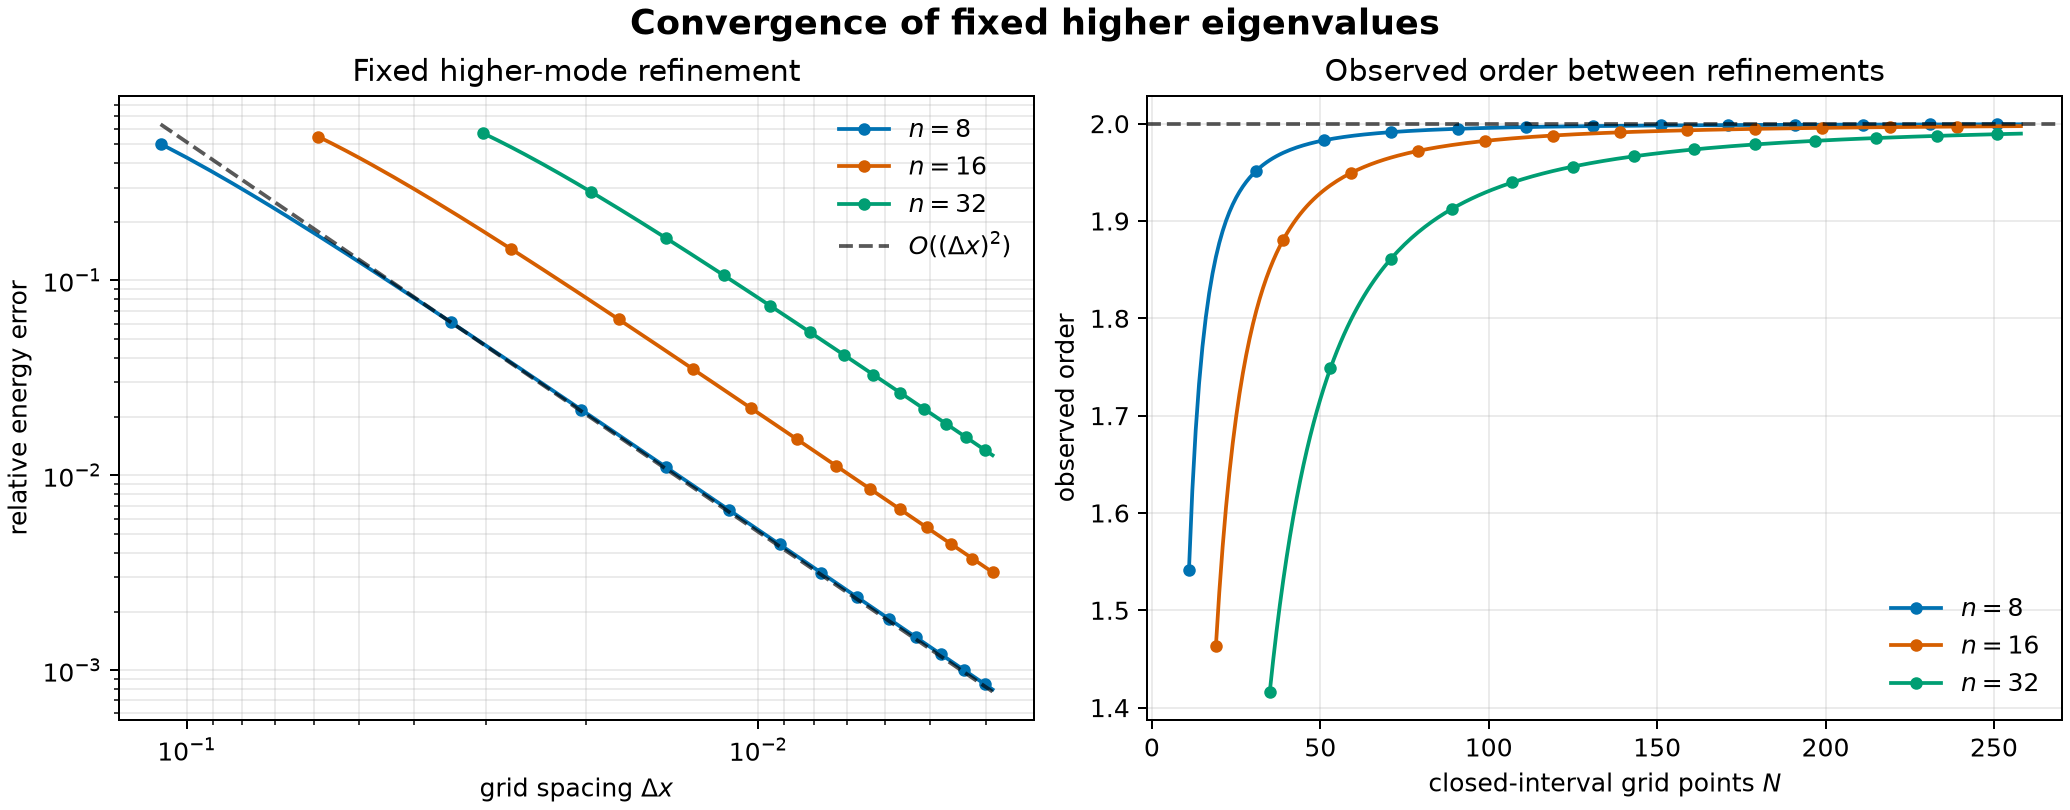
\includegraphics[width=0.94\linewidth]{higher-mode-convergence.png}
\caption{Relative energy error and observed refinement order for selected fixed
higher modes. The second-order regime appears later as the mode index increases.}
\label{fig:higher-mode-convergence}
\end{figure}

\subsection{Residual geometry records the comparison being made}

For the box model, the finite Hamiltonian is the finite Dirichlet kinetic matrix,
$\mat{H}_{\Delta x}=\mat{T}_{\mathrm{D},\Delta x}$. The consistently compressed
residual defined in Equation~\eqref{eq:method-consistent-residual} therefore satisfies
\begin{equation}
 \mat{R}_{\mathrm{cons}}=\mat{0}.
 \label{eq:consistent-compression}
\end{equation}
This is the reduced physical potential for the declared finite model. The blank left
panel of Figure~\ref{fig:residuals} is therefore a substantive result: applying the
same projection to both terms preserves the exact zero-potential identity.

The unmatched residual in Equation~\eqref{eq:method-unmatched-residual} instead
satisfies
\begin{equation}
 \mat{R}_{\mathrm{un}}
 =-\mat{Q}_M\mat{T}_{\mathrm{D},\Delta x}\mat{Q}_M.
 \label{eq:unmatched-compression}
\end{equation}
The middle panel of Figure~\ref{fig:residuals} consequently reproduces the structured
discarded kinetic sector. Its nonzero diagonal and near-diagonal pattern is not a newly
inferred potential; it is the visible consequence of subtracting an uncompressed
operator from a compressed one.

The right panel isolates a third geometry. Changing from the Dirichlet to the cyclic
closure modifies only the two corner couplings, so the residual is sparse and
boundary-localized. The residual therefore isolates the effect of changing the
boundary condition in the discrete operator; it is not a potential-energy term.

\begin{figure}[ht]
\centering
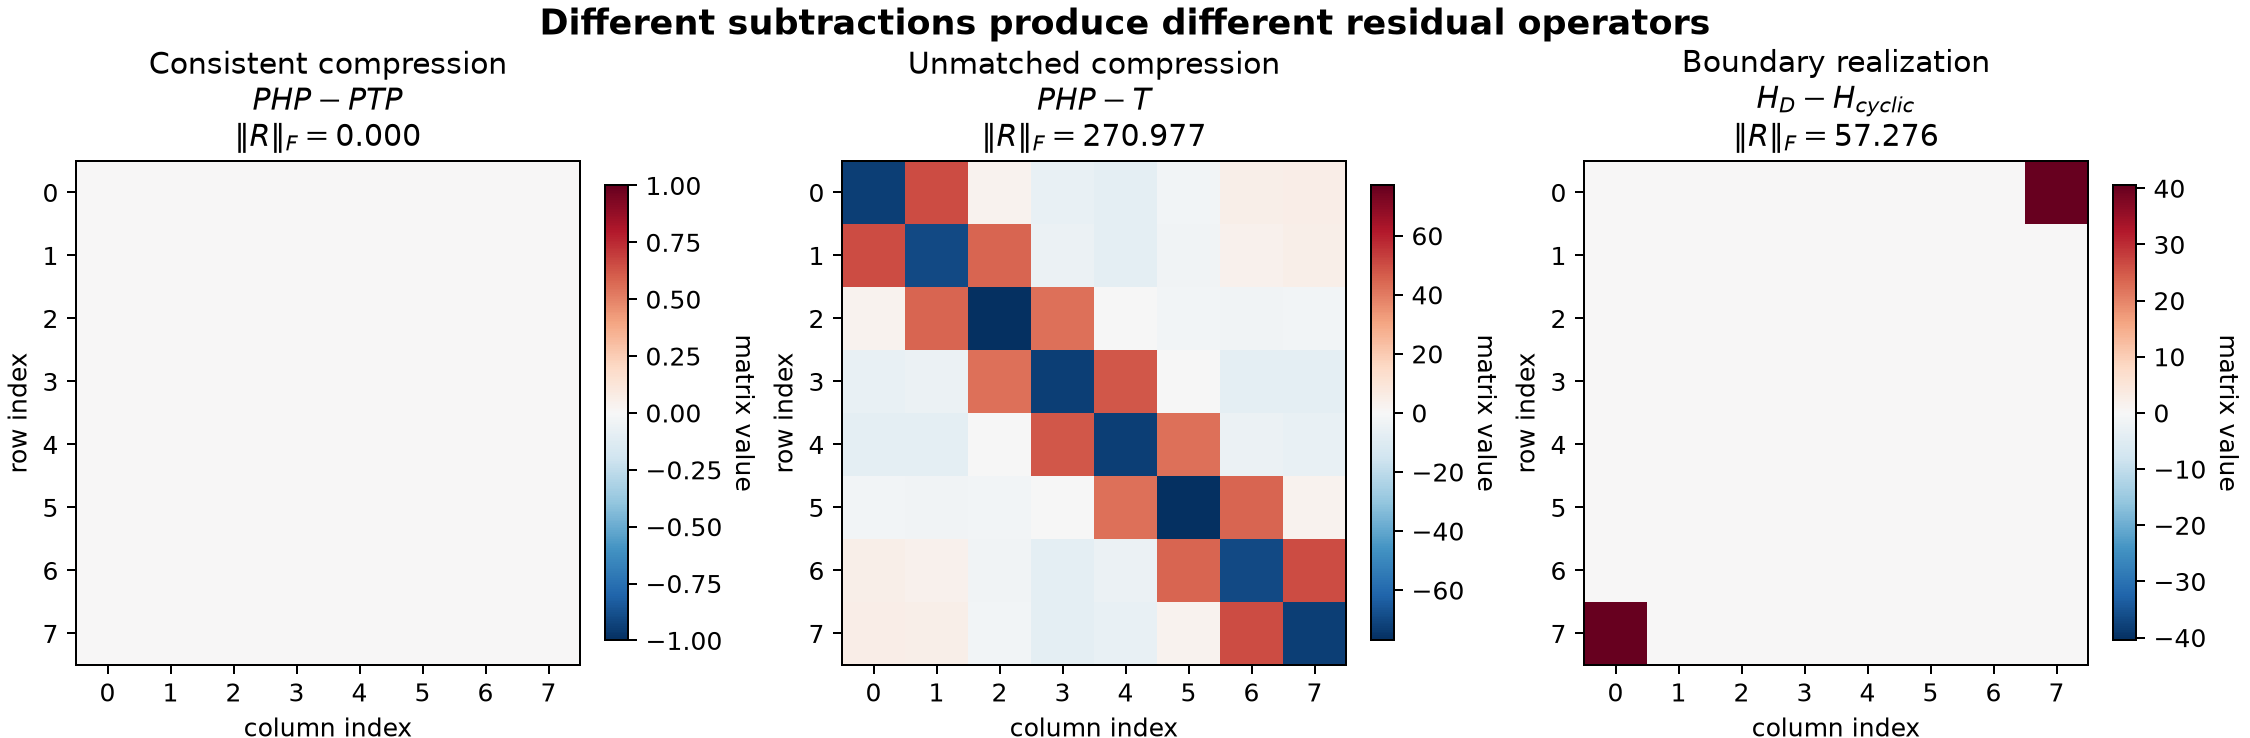
\includegraphics[width=\linewidth]{residual-matrices.png}
\caption{Three residual constructions. Consistent compression gives zero; unmatched
compression retains the discarded kinetic sector; changing the boundary closure
changes two corner couplings.}
\label{fig:residuals}
\end{figure}

Figure~\ref{fig:operator-residual-norms} shows why the heatmap geometry must accompany
a scalar norm. With fixed $M$, the unmatched residual contains the entire high-energy
sector. Its normalized spectral norm is therefore one, and its Frobenius and
maximum-entry ratios approach one as the grid grows: almost all of the expanding
operator lies outside the fixed retained subspace. The boundary residual behaves in
the opposite way. Its two corner entries become negligible in the global Frobenius
ratio, while its spectral ratio approaches one quarter and its maximum-entry ratio
remains one half. No contradiction is present; the three norms ask different
questions of the same sparse boundary perturbation.

\begin{figure}[!htbp]
\centering
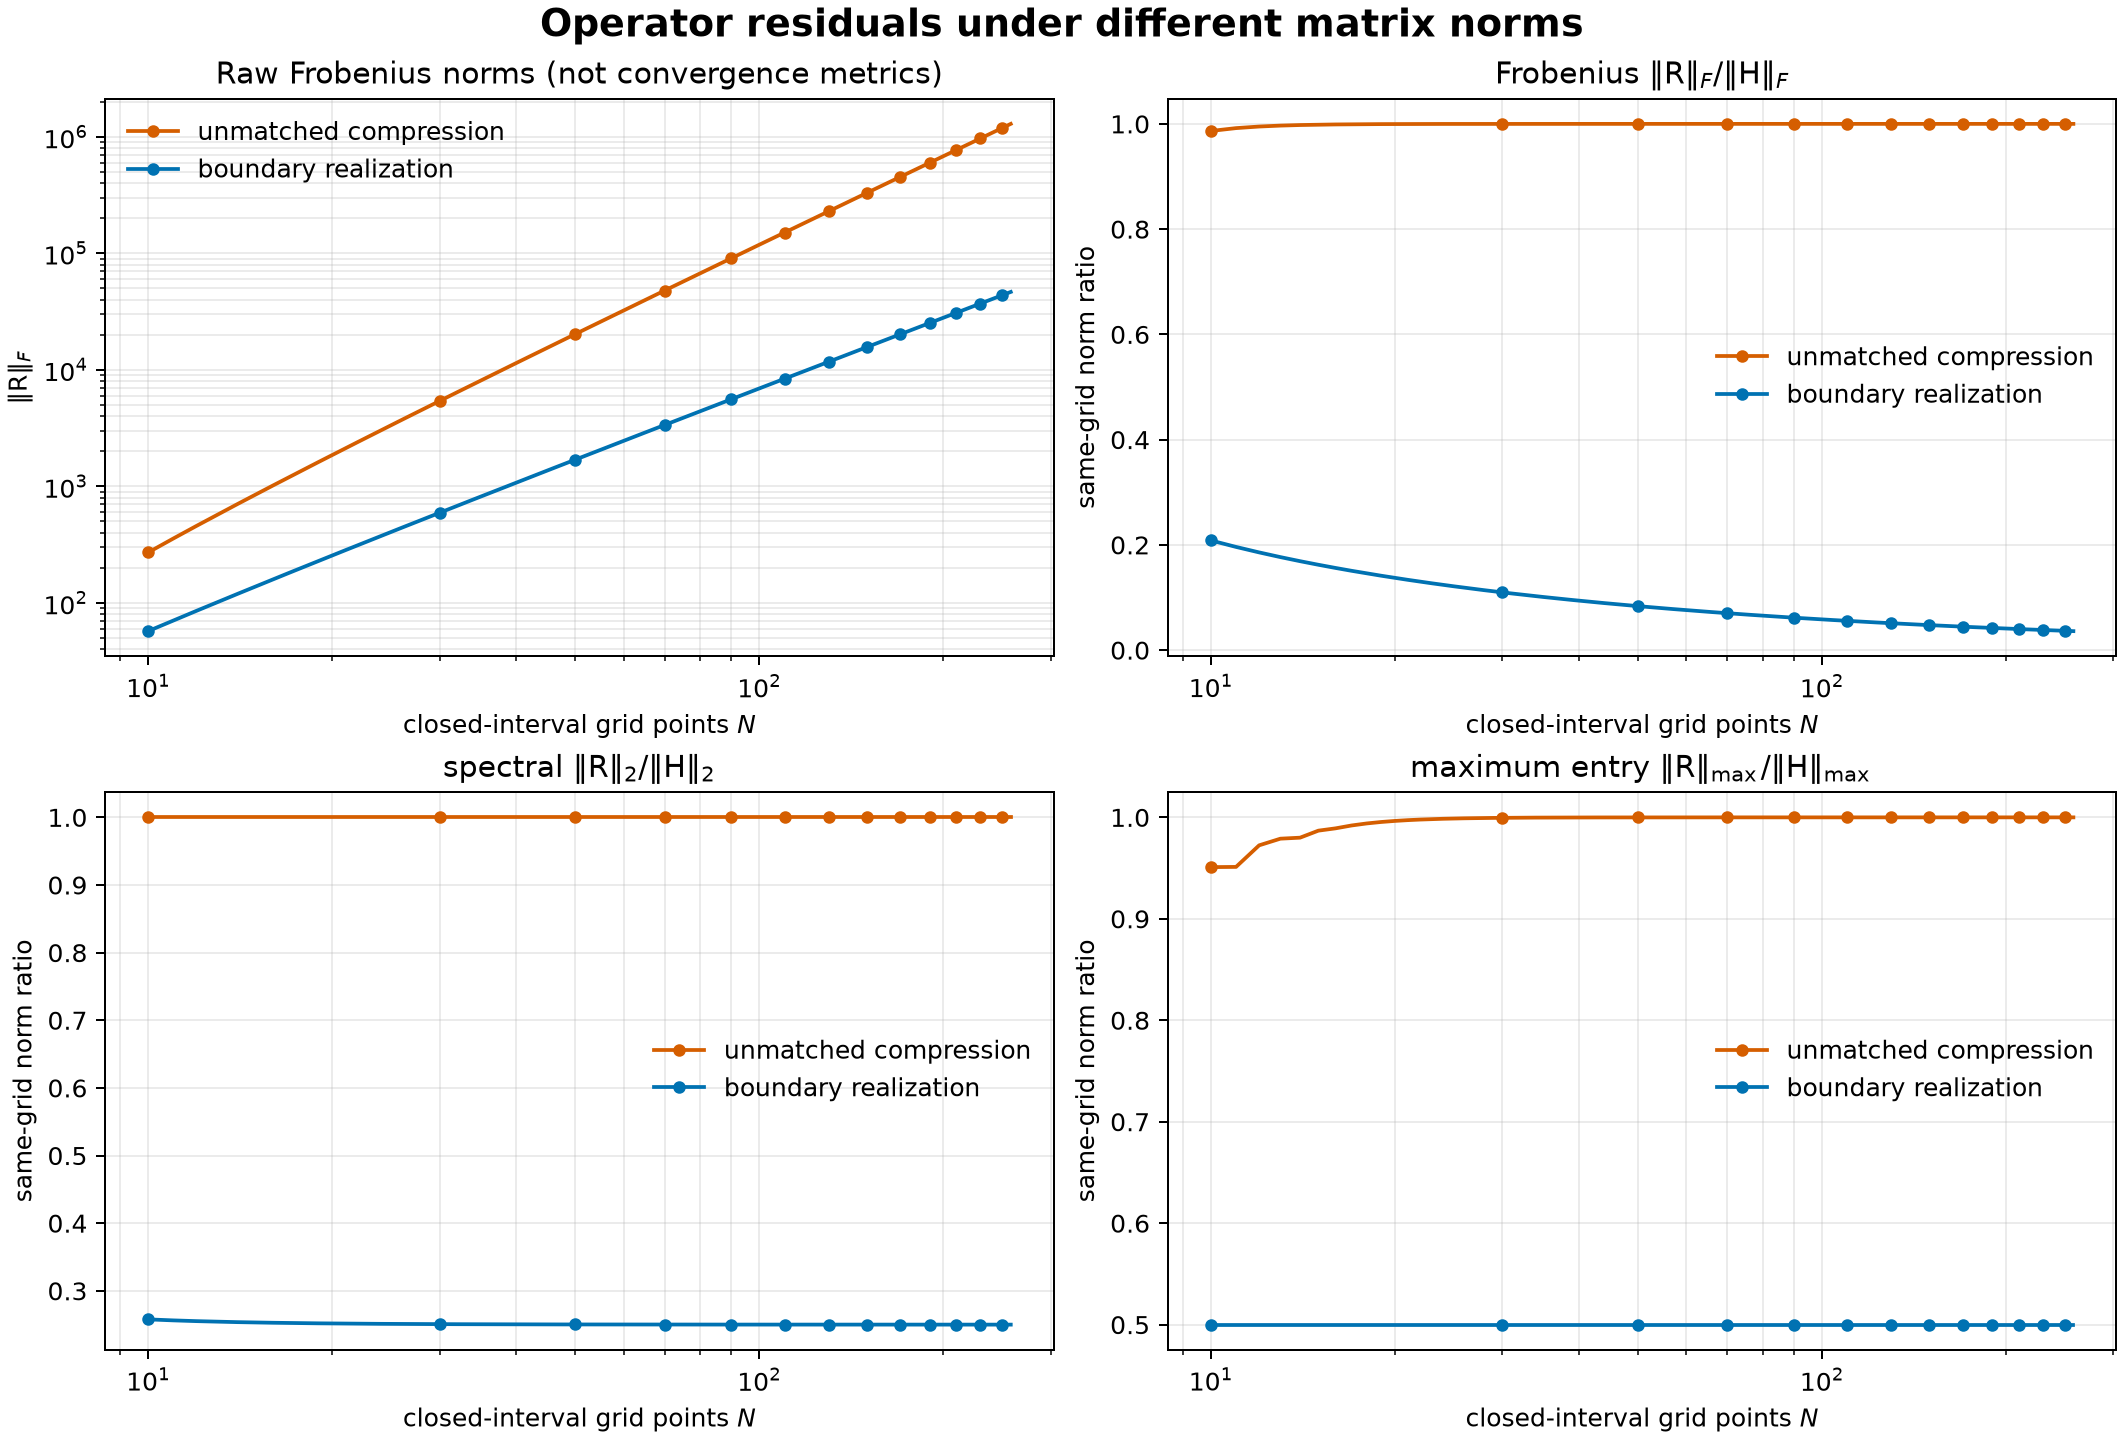
\includegraphics[width=\linewidth]{operator-residual-norms.png}
\caption{Raw and same-grid-normalized residual norms for every closed-interval grid
size $N=10,11,\ldots,258$. The panels demonstrate that norm choice is part of the
diagnostic definition.}
\label{fig:operator-residual-norms}
\end{figure}

\FloatBarrier
\subsection{Identifiability comes from the model class}

Let $\mathcal K$ and $\mathcal V$ be admissible classes for the kinetic and potential
parts of a matrix $\mat{H}$. The compatible decompositions form the fiber
\begin{equation}
 \mathcal D_{\mat{H}}(\mathcal K,\mathcal V)
 =\{(\mat{T},\mat{V}):\mat{T}\in\mathcal K,\
 \mat{V}\in\mathcal V,\ \mat{H}=\mat{T}+\mat{V}\}.
\end{equation}
A sufficient global uniqueness condition is
\begin{equation}
 (\mathcal K-\mathcal K)\cap(\mathcal V-\mathcal V)=\{0\}.
 \label{eq:identifiability}
\end{equation}
Without such a restriction, the matrix alone does not select one additive split.

The retained calculation starts from
$\mat{H}_{\mathrm{red}}=\mat{T}_{\mathrm{D},\mathrm{red}}+\mat{0}$. For a declared
real-symmetric shift $\mat{K}$, the same matrix also satisfies
\begin{equation}
 \mat{H}_{\mathrm{red}}
 =(\mat{T}_{\mathrm{D},\mathrm{red}}-\mat{K})+\mat{K}.
\end{equation}
The equality is algebraically exact, but it does not make $\mat{K}$ a physical
potential.
Figure~\ref{fig:identifiability} shows what the successive model classes contribute.
Scalar and diagonal classes leave most of the illustrative shift unexplained because
they cannot represent its off-diagonal structure. Allowing nearest-neighbor couplings
captures most of that structure, while the unrestricted real-symmetric class fits
exactly by construction. The monotone reduction in residual is therefore not evidence
that the unrestricted decomposition is more physical. It records only the increasing
expressiveness of the admissible class; physical identifiability requires that class to
be justified independently.

\begin{figure}[ht]
\centering
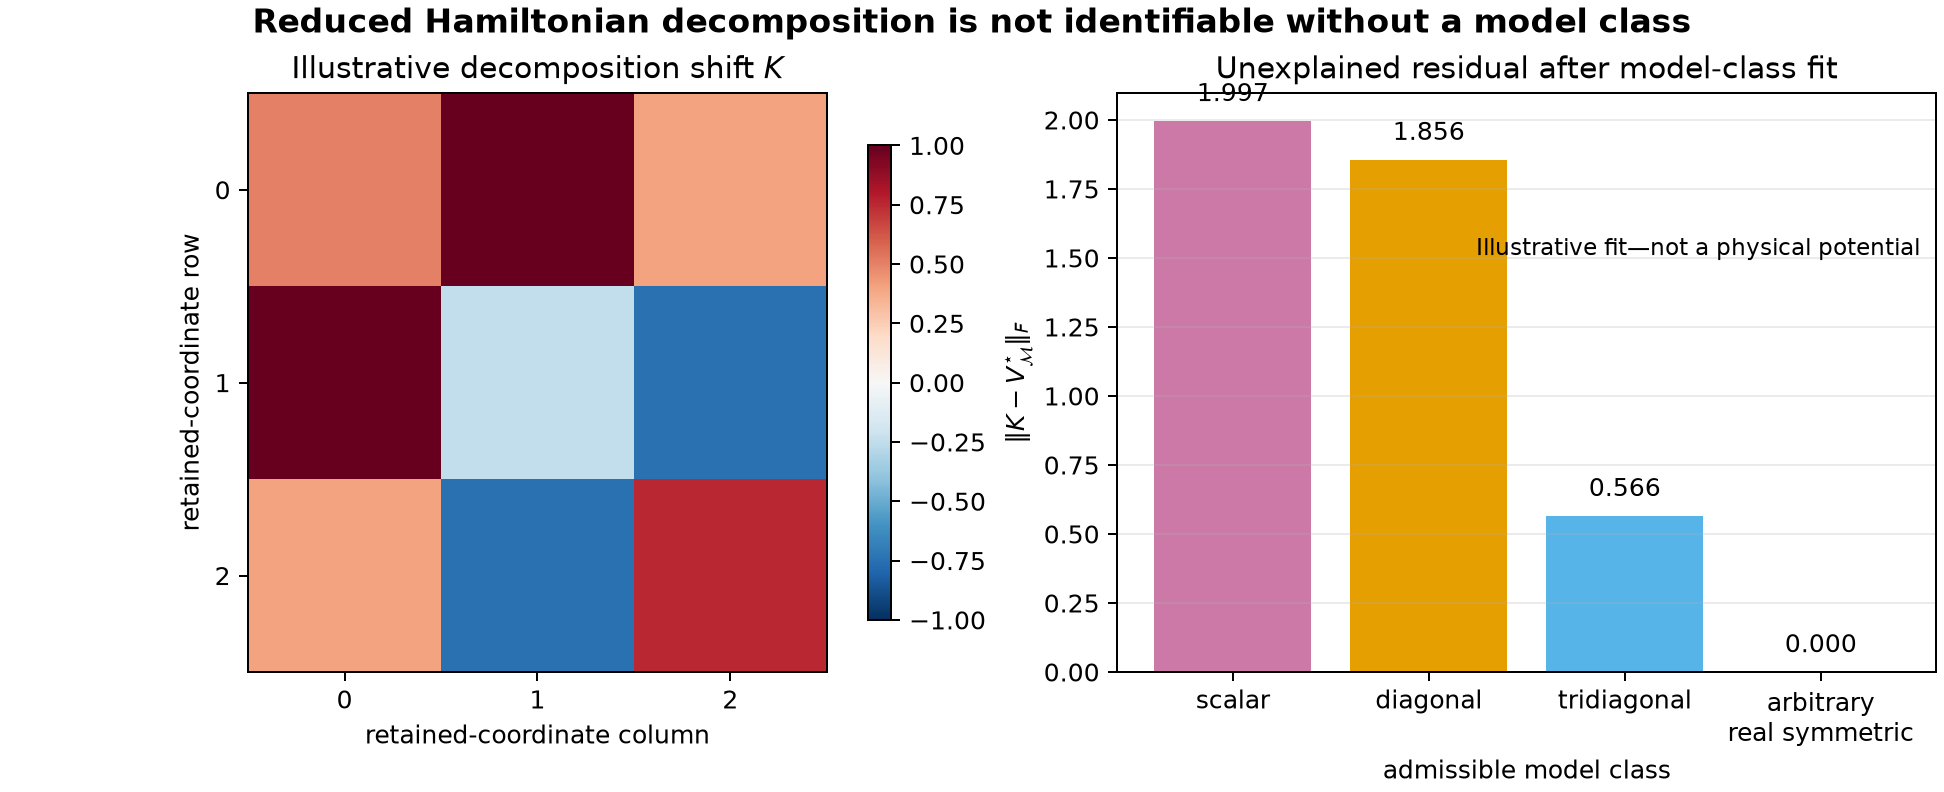
\includegraphics[width=0.94\linewidth]{identifiability-model-classes.png}
\caption{An illustrative decomposition shift and its best fit in four model classes.
Exact representability in the unrestricted class does not establish a physical
interpretation.}
\label{fig:identifiability}
\end{figure}

\subsection{Implications for reduced-model diagnostics}

Taken together, the results establish three distinct levels of assessment. Algebraic
closure asks whether the represented eigenproblem, projector, and compression
identities are satisfied. Continuum approximation asks whether the represented modes
resolve the wavelengths of interest. Physical interpretation asks whether a residual
or additive decomposition belongs to a justified model class. Success at one level
does not establish success at the next.

The residual study also shows that a norm cannot supply meaning that is absent from
the operator being measured. Consistent compression, unmatched compression, and a
change of boundary condition produce different residual matrices before any norm is
chosen. Frobenius, spectral, and maximum-entry norms then expose different global,
action-based, and coordinate-local properties of those matrices. Both the residual
definition and its representation must therefore precede scalar comparison.

PIAB1D is a calibration case because its retained trial space is an exact spectral
subspace. More general trial spaces need not be invariant, so projector defects,
leakage, analytical residuals, and operator-comparison errors can become independent
channels rather than roundoff-level identities. The separation demonstrated here
provides a controlled reference for interpreting those channels in less structured
models.

\section{Verification, formalization, and limitations}

The calculation is checked at three distinct levels. JSON schemas check document
structure. Numerical verification scripts recompute finite formulas and algebraic
relationships from retained data. Formal numerical analysis can extend much farther:
prior work has mechanized a centered finite-difference wave solver from analytical
error through its C implementation \cite{boldoEtAl2013,boldoEtAl2014}, and the Lax
equivalence theorem for finite-difference schemes has been formalized in Coq
\cite{tekriwalDuraisamyJeannin2021}. The separate Lean~4 development used here has a
more limited target. It uses mathlib \cite{demouraUllrich2021,mathlib2020} to prove
exact statements about finite Dirichlet recurrences, matrix eigenpairs, orthogonal
compression, decomposition nonuniqueness, and finite model-class fitting.

These levels are complementary but not interchangeable. The Lean proofs do not
certify NumPy or SciPy execution, serialized bytes, binary64 rounding, plotted
figures, or the continuum limit. The numerical calculations do not prove general
theorems. The verification scripts are separate code paths in the same repository;
they are not external replications.

The model itself is also intentionally limited. No experimental system is identified,
no parameters are calibrated to a material, and no uncertainty model is introduced.
Agreement with the analytical particle-in-a-box spectrum verifies the implementation
against the same mathematical model. It is not physical validation.

\section{Software and data availability}

The software and documentation supporting this work are maintained in
\href{https://github.com/eragasa/ksdft2effmass}{\code{ksdft2effmass}}. The calculation
uses components from the ProjectKoios system of libraries developed by the author,
including
\href{https://github.com/eragasa/projectkoios-physkit}{\code{projectkoios-physkit}}
and
\href{https://github.com/eragasa/projectkoios-optimization}{\code{projectkoios-optimization}},
whose \path{projectkoios.numerics.quadrature} package supplies the unit-free rule.
These repositories are publicly available under the
\href{https://www.apache.org/licenses/LICENSE-2.0}{Apache License 2.0}.

The demonstrations, retained numerical results, verification programs, and plotting
sources are preserved together under the stable calculation owner
\begin{center}
\url{https://github.com/eragasa/ksdft2effmass/tree/main/calculations/piab1d}
\end{center}
File-level provenance and byte integrity are recorded in the accompanying
\code{SHA256SUMS} manifest. At release, the archived repository snapshot will also be
identified by its immutable Git commit identifier. The Git commit identifies the
source snapshot, whereas the SHA-256 manifest identifies the retained artifact bytes.

\section{Conclusion}

The one-dimensional particle in a box gives an unusually clean view of spectral
reduction. The finite matrix is solved accurately, its lowest eigenspace is invariant,
and its reduced Hamiltonian is known exactly in spectral coordinates. The remaining
spectral discrepancy is finite-difference dispersion: it is second order for fixed
resolved modes but remains large near the top of a growing spectrum.

The same calculation also shows why residual operators require careful definitions.
Consistent compression, unmatched compression, and a change of boundary closure lead
to different matrices with different interpretations. An additive decomposition is
similarly meaningful only relative to an admissible model class. The contribution is
the integration of these distinctions with independently recomputed numerical
artifacts and a bounded formal crosswalk, not novelty of the box solution, the stencil,
or spectral projection. As the first stage of the planned diagnostic sequence, this
calculation establishes the reference case against which later spatial truncation,
periodic, lattice, multiband, and first-principles reductions can be interpreted.

\bibliographystyle{plain}
\bibliography{references}

\clearpage
\appendix
\section*{Supplemental material}
\addcontentsline{toc}{section}{Supplemental material}

\section{Exact finite identities underlying the diagnostics}
\label{app:exact-identities}

This appendix proves the finite identities used to interpret the numerical figures.
The proofs concern exact real matrices and exact scalar formulas. They do not certify
the binary64 calculations, serialized results, or plotting programs.

\subsection{Monotonicity of the retained canonical weight}

Let $d=N-2$ and define the represented canonical probabilities
\begin{equation}
 p_n^{(\beta,\Delta x)}
 =\frac{\exp(-\beta E_{n,\Delta x})}{Z_{\Delta x}},
 \qquad n=1,\ldots,d.
\end{equation}
Every probability is strictly positive, and
$w_{>M}^{(\beta,\Delta x)}=\sum_{n=M+1}^{d}p_n^{(\beta,\Delta x)}$.
For $M<d$,
\begin{equation}
 w_{>(M+1)}^{(\beta,\Delta x)}
 =w_{>M}^{(\beta,\Delta x)}-p_{M+1}^{(\beta,\Delta x)}
 <w_{>M}^{(\beta,\Delta x)}.
 \label{eq:appendix-tail-recurrence}
\end{equation}
Moreover, $w_{>d}^{(\beta,\Delta x)}=0$. Hence the feasible set in
Equation~\eqref{eq:retained-dimension-rule} is nonempty for every $\tau\geq0$, and its
smallest element is unique. If $\tau_1\leq\tau_2$, every dimension feasible for
$\tau_1$ is feasible for $\tau_2$, so
\begin{equation}
 M_{\star}(N,\beta,\tau_2)
 \leq M_{\star}(N,\beta,\tau_1).
\end{equation}
Thus $M_{\star}$ is a nonincreasing integer-valued step function of the a priori
tolerance. Its transitions occur at the finite set of canonical tail weights.
\hfill$\square$

\paragraph{Scientific interpretation.}
The inverse temperature $\beta$ identifies the energy range populated by the declared
canonical ensemble, while $\tau$ specifies how much of that population may be omitted.
The rule therefore converts a scientific resolution requirement into the smallest
state count that satisfies it. A plateau means that the selected model size is stable
to changes of $\tau$ within that interval; it does not make the choice independent of
the ensemble or tolerance.

\subsection{Exact eigensystem of the Dirichlet difference matrix}

Set $d=N-2$, $\Delta x=L/(d+1)$, and
\begin{equation}
 a=\frac{\hbar^2}{2m(\Delta x)^2}.
\end{equation}
Let $\mat{T}_d$ be the $d\times d$ matrix with diagonal entries $2$, first
off-diagonal entries $-1$, and all other entries zero, so that
$\mat{H}_{\Delta x}=a\mat{T}_d$. For $n=1,\ldots,d$, define
\begin{equation}
 \theta_n=\frac{n\pi}{d+1},
 \qquad
 (\vect{u}_n)_j
 =\sqrt{\frac{2}{d+1}}\sin(j\theta_n),
 \quad j=1,\ldots,d.
 \label{eq:appendix-discrete-sine-mode}
\end{equation}
The ghost values at $j=0$ and $j=d+1$ vanish. At every interior coordinate,
\begin{align}
 (\mat{T}_d\vect{u}_n)_j
 &=2(\vect{u}_n)_j-(\vect{u}_n)_{j-1}-(\vect{u}_n)_{j+1} \\
 &=2(1-\cos\theta_n)(\vect{u}_n)_j \\
 &=4\sin^2\!\left(\frac{\theta_n}{2}\right)(\vect{u}_n)_j.
\end{align}
The discrete sine orthogonality identity
\begin{equation}
 \sum_{j=1}^{d}\sin(j\theta_n)\sin(j\theta_m)
 =\frac{d+1}{2}\,\delta_{nm}
 \label{eq:appendix-discrete-sine-orthogonality}
\end{equation}
follows by applying the product-to-sum formula and evaluating the two finite cosine
sums. Therefore the vectors in Equation~\eqref{eq:appendix-discrete-sine-mode} form an
orthonormal basis, and
\begin{equation}
 \mat{H}_{\Delta x}\vect{u}_n
 =E_{n,\Delta x}\vect{u}_n,
 \qquad
 E_{n,\Delta x}
 =4a\sin^2\!\left(\frac{n\pi}{2(d+1)}\right).
 \label{eq:appendix-discrete-eigenpair}
\end{equation}
Writing $\mat{U}=[\vect{u}_1\ \cdots\ \vect{u}_d]$ and
$\mat{D}_{\Delta x}=\operatorname{diag}(E_{1,\Delta x},\ldots,E_{d,\Delta x})$
gives the exact reconstruction
\begin{equation}
 \mat{U}^{\mathsf T}\mat{U}=\mat{I},
 \qquad
 \mat{H}_{\Delta x}
 =\mat{U}\mat{D}_{\Delta x}\mat{U}^{\mathsf T}.
 \label{eq:appendix-exact-reconstruction}
\end{equation}
\hfill$\square$

\paragraph{Scientific interpretation.}
The vectors $\vect{u}_n$ are the standing-wave shapes permitted by two impenetrable
ends, sampled on the interior grid. Their increasing node count corresponds to
shorter wavelength and higher kinetic energy. Orthogonality makes these modes
independent coordinates of the finite model, and reconstruction shows that they
exhaust that model. The result is exact for the discrete Hamiltonian; it does not by
itself establish that every discrete energy accurately represents the continuum box.

\subsection{Exact identities for spectral reduction}

Let $\mat{U}_M=[\vect{u}_1\ \cdots\ \vect{u}_M]$,
$\mat{D}_M=\operatorname{diag}(E_{1,\Delta x},\ldots,E_{M,\Delta x})$, and
$\mat{P}_M=\mat{U}_M\mat{U}_M^{\mathsf T}$. Orthonormality and
$\mat{H}_{\Delta x}\mat{U}_M=\mat{U}_M\mat{D}_M$ imply
\begin{align}
 \mat{P}_M^2
 &=\mat{U}_M(\mat{U}_M^{\mathsf T}\mat{U}_M)\mat{U}_M^{\mathsf T}
 =\mat{P}_M, \\
 \mat{H}_{\mathrm{red}}
 &=\mat{U}_M^{\mathsf T}\mat{H}_{\Delta x}\mat{U}_M
 =\mat{D}_M, \\
 \mat{P}_M\mat{H}_{\Delta x}\mat{P}_M
 &=\mat{U}_M\mat{D}_M\mat{U}_M^{\mathsf T}.
 \label{eq:appendix-reduction-identities}
\end{align}
For $\mat{Q}_M=\mat{I}-\mat{P}_M$,
\begin{equation}
 \mat{Q}_M\mat{H}_{\Delta x}\mat{U}_M
 =(\mat{I}-\mat{P}_M)\mat{U}_M\mat{D}_M
 =\mat{0}.
 \label{eq:appendix-zero-leakage}
\end{equation}
Equations~\eqref{eq:appendix-exact-reconstruction}--
\eqref{eq:appendix-zero-leakage} show that
$\delta_{\mathrm{rec}}$, $\delta_{\mathrm{idem}}$,
$\delta_{\mathrm{coord}}$, $\delta_{\mathrm{embed}}$, and
$\delta_{\mathrm{leak}}$ vanish in exact arithmetic. Their nonzero calculated values
therefore measure finite-precision closure of these identities, not continuum error.
\hfill$\square$

\paragraph{Scientific interpretation.}
Retaining exact eigenvectors selects an invariant low-energy sector of the represented
box. Applying the finite Hamiltonian to a retained state cannot generate a component
outside that sector, so the leakage is exactly zero before floating-point evaluation.
This makes PIAB1D a calibration case: nonzero leakage in a general trial basis would
measure genuine coupling to omitted represented states, whereas here it can only
measure numerical closure. Neither outcome determines the continuum discretization
error.

\subsection{Pointwise convergence and full-spectrum dispersion}

The continuum energy can be written using the same scale $a$ as
\begin{equation}
 E_n
 =\frac{\hbar^2\pi^2n^2}{2mL^2}
 =4a z_{n,d}^2,
 \qquad
 z_{n,d}=\frac{n\pi}{2(d+1)}.
\end{equation}
Combining this expression with Equation~\eqref{eq:appendix-discrete-eigenpair} gives
\begin{equation}
 \frac{E_{n,\Delta x}}{E_n}
 =\left(\frac{\sin z_{n,d}}{z_{n,d}}\right)^2,
 \qquad
 \epsilon_{n,N}
 =1-\left(\frac{\sin z_{n,d}}{z_{n,d}}\right)^2.
 \label{eq:appendix-exact-dispersion-error}
\end{equation}
For fixed $n$, the Taylor expansion at the origin yields
\begin{equation}
 \epsilon_{n,N}
 =\frac{z_{n,d}^2}{3}+O(z_{n,d}^4)
 =\frac{n^2\pi^2}{12L^2}(\Delta x)^2+O((\Delta x)^4).
 \label{eq:appendix-fixed-mode-order}
\end{equation}
This proves second-order convergence for every fixed mode. In contrast, suppose that
$n/(d+1)\to q$ with $q\in(0,1]$. Then
\begin{equation}
 \epsilon_{n,N}\longrightarrow
 1-\left[
 \frac{\sin(\pi q/2)}{\pi q/2}
 \right]^2>0,
 \label{eq:appendix-fractional-mode-limit}
\end{equation}
because $\sin x<x$ for $x>0$. Thus refinement does not give uniform relative spectral
convergence over a mode set whose dimension grows with the grid. This is the exact
curve onto which the full-spectrum results collapse.
\hfill$\square$

\paragraph{Scientific interpretation.}
Holding $n$ fixed means holding a physical standing-wave pattern fixed while placing
more grid points across it; the wavelength is increasingly well resolved. Holding
$q=n/(d+1)$ fixed instead keeps the wavelength at a fixed fraction of the grid scale,
so the number of points per oscillation does not improve. Grid refinement then adds
new short-wavelength states without making those states better continuum
approximations. This is why low-energy observables may converge even though the full
growing spectrum does not converge uniformly.

\subsection{Compression and boundary residuals}

Because $\mat{H}_{\Delta x}=\mat{T}_{\mathrm{D},\Delta x}$, consistent compression
vanishes immediately. Spectral projectors commute with the Hamiltonian, so
\begin{equation}
 \mat{H}_{\Delta x}
 =\mat{P}_M\mat{H}_{\Delta x}\mat{P}_M
 +\mat{Q}_M\mat{H}_{\Delta x}\mat{Q}_M.
\end{equation}
The unmatched residual is therefore
\begin{equation}
 \mat{R}_{\mathrm{un}}
 =-\mat{Q}_M\mat{H}_{\Delta x}\mat{Q}_M
 =-\sum_{n=M+1}^{d}E_{n,\Delta x}
   \vect{u}_n\vect{u}_n^{\mathsf T}.
 \label{eq:appendix-unmatched-spectral-form}
\end{equation}
Since the energies are positive and increasing,
\begin{equation}
 \lVert\mat{R}_{\mathrm{un}}\rVert_2=E_{d,\Delta x},
 \qquad
 \lVert\mat{R}_{\mathrm{un}}\rVert_{\fro}^2
 =\sum_{n=M+1}^{d}E_{n,\Delta x}^2.
 \label{eq:appendix-unmatched-norms}
\end{equation}
Hence the Hamiltonian-normalized spectral norm is exactly one whenever $M<d$.
For fixed $M$, the normalized Frobenius norm approaches one as $d$ grows because the
finite retained sum becomes negligible relative to the full spectral square sum.

For the cyclic reference, let $\vect{e}_1$ and $\vect{e}_d$ denote the first and last
coordinate vectors and assume $d\geq2$. The cyclic matrix adds the two corner
couplings $-a$, so
\begin{equation}
 \mat{H}_{\mathrm{cyclic},\Delta x}
 =\mat{H}_{\mathrm{D},\Delta x}
 -a(\vect{e}_1\vect{e}_d^{\mathsf T}
    +\vect{e}_d\vect{e}_1^{\mathsf T}),
\end{equation}
and therefore
\begin{equation}
 \mat{R}_{\mathrm{bc}}
 =a(\vect{e}_1\vect{e}_d^{\mathsf T}
    +\vect{e}_d\vect{e}_1^{\mathsf T}).
 \label{eq:appendix-boundary-residual}
\end{equation}
This matrix has two nonzero entries and acts on
$\operatorname{span}\{\vect{e}_1,\vect{e}_d\}$ as
$\left[\begin{smallmatrix}0&a\\a&0\end{smallmatrix}\right]$. Consequently,
\begin{equation}
 \lVert\mat{R}_{\mathrm{bc}}\rVert_{\fro}=\sqrt{2}\,a,
 \qquad
 \lVert\mat{R}_{\mathrm{bc}}\rVert_2=a,
 \qquad
 \lVert\mat{R}_{\mathrm{bc}}\rVert_{\max}=a.
 \label{eq:appendix-boundary-raw-norms}
\end{equation}
Counting the entries of the Dirichlet tridiagonal matrix and using its largest
eigenvalue gives
\begin{equation}
 \lVert\mat{H}_{\Delta x}\rVert_{\fro}=a\sqrt{6d-2},
 \quad
 \lVert\mat{H}_{\Delta x}\rVert_2
 =4a\cos^2\!\left(\frac{\pi}{2(d+1)}\right),
 \quad
 \lVert\mat{H}_{\Delta x}\rVert_{\max}=2a.
\end{equation}
The normalized boundary diagnostics are therefore
\begin{equation}
 \eta_{\fro}(\mat{R}_{\mathrm{bc}})=\frac{1}{\sqrt{3d-1}},
 \qquad
 \eta_2(\mat{R}_{\mathrm{bc}})
 =\frac{1}{4\cos^2(\pi/[2(d+1)])},
 \qquad
 \eta_{\max}(\mat{R}_{\mathrm{bc}})=\frac12.
 \label{eq:appendix-boundary-normalized-norms}
\end{equation}
Thus the Frobenius ratio tends to zero, the spectral ratio tends to one quarter, and
the maximum-entry ratio remains one half. The distinct trends in
Figure~\ref{fig:operator-residual-norms} follow from the matrix geometry rather than
from conflicting numerical results.
\hfill$\square$

\paragraph{Scientific interpretation.}
The unmatched residual is dominated by the high-energy states deliberately excluded
from the reduced model; calling it a potential would mistake omitted kinetic content
for new physics. The boundary residual has a different origin. Connecting the first
and last coordinates changes an open box into a finite ring-like closure, and the two
corner entries record only that boundary choice. Its norm describes the size of the
boundary modification in a chosen matrix metric, not the strength of a continuum
potential.

\subsection{Identifiability and Frobenius-optimal model classes}

Suppose
$\mat{H}=\mat{T}_1+\mat{V}_1=\mat{T}_2+\mat{V}_2$ with
$\mat{T}_1,\mat{T}_2\in\mathcal K$ and
$\mat{V}_1,\mat{V}_2\in\mathcal V$. Rearrangement gives
\begin{equation}
 \mat{T}_1-\mat{T}_2
 =\mat{V}_2-\mat{V}_1
 \in(\mathcal K-\mathcal K)\cap(\mathcal V-\mathcal V).
\end{equation}
If the intersection is $\{\mat{0}\}$, then
$\mat{T}_1=\mat{T}_2$ and $\mat{V}_1=\mat{V}_2$. This proves the uniqueness condition
in Equation~\eqref{eq:identifiability}. Conversely, any nonzero matrix in the
intersection supplies two distinct admissible decompositions of the same sum, so the
condition also characterizes global uniqueness over the declared classes.

The model-class fits in Figure~\ref{fig:identifiability} are orthogonal projections in
the Frobenius inner product. For a coordinate-support class $\mathcal C$, let
$\Pi_{\mathcal C}\mat{K}$ retain the permitted entries and set all others to zero.
The supported and omitted entries are disjoint, so every
$\mat{V}\in\mathcal C$ satisfies the Pythagorean identity
\begin{equation}
 \lVert\mat{K}-\mat{V}\rVert_{\fro}^2
 =\lVert\mat{K}-\Pi_{\mathcal C}\mat{K}\rVert_{\fro}^2
 +\lVert\Pi_{\mathcal C}\mat{K}-\mat{V}\rVert_{\fro}^2.
 \label{eq:appendix-model-fit-pythagorean}
\end{equation}
Hence the diagonal and tridiagonal minimizers are obtained by retaining, respectively,
the diagonal entries and the entries with $|i-j|\leq1$. For the scalar-identity class,
\begin{equation}
 \lVert\mat{K}-c\mat{I}\rVert_{\fro}^2
 =\sum_i(K_{ii}-c)^2+\sum_{i\neq j}K_{ij}^2
\end{equation}
is minimized at $c=\operatorname{tr}(\mat{K})/M$. Finally, because the illustrative
shift is itself real symmetric, the unrestricted real-symmetric class contains
$\mat{K}$ and has zero residual. These are statements about approximation within the
declared matrix classes; they do not assign physical meaning to the fitted matrices.
\hfill$\square$

\paragraph{Scientific interpretation.}
An observed reduced Hamiltonian does not reveal, by itself, which entries should be
called kinetic and which should be called potential. A more expressive matrix class
will always fit at least as well, and an unrestricted class fits exactly by definition.
Scientific identification therefore requires independently justified structure---for
example locality, symmetry, known interactions, or a prescribed basis---rather than
fit quality alone.

\section{Machine-checked crosswalk}
\label{app:formal-crosswalk}

The companion formalization is maintained in
\href{https://github.com/eragasa/projectkoios-formal}{
\code{github.com/eragasa/projectkoios-formal}}. The calculation sources are maintained
in
\href{https://github.com/eragasa/ksdft2effmass}{
\code{github.com/eragasa/ksdft2effmass}}. Table~\ref{tab:formal-crosswalk} identifies
the machine-checked theorem families corresponding to the exact finite arguments
above. The GitHub formalization and this numerical repository remain separate evidence
owners.

\begin{table}[!htbp]
\centering
\small
\begin{tabular}{@{}
>{\raggedright\arraybackslash}p{0.32\linewidth}
>{\raggedright\arraybackslash}p{0.28\linewidth}
>{\raggedright\arraybackslash}p{0.31\linewidth}@{}}
\toprule
Appendix statement & Formal theorem identifiers & Boundary of the formal result \\
\midrule
Canonical finite Dirichlet mode and discrete eigenvalue
 & PIAB1D-SPECTRUM-THM-015, PIAB1D-SPECTRUM-THM-016
 & Exact finite eigenpair; no binary64 or continuum-completeness claim \\
Dirichlet--cyclic corner relation and support
 & PIAB1D-BOUNDARY-THM-001, PIAB1D-BOUNDARY-THM-002,
   PIAB1D-BOUNDARY-THM-004
 & Exact finite matrix identity and periodic specialization \\
Consistent and unmatched orthogonal compression
 & QM-COMPRESSION-THM-001, QM-COMPRESSION-THM-002
 & Exact under the declared idempotency and commutation hypotheses \\
Shifted decomposition nonuniqueness
 & QM-IDENTIFIABILITY-THM-001, QM-IDENTIFIABILITY-THM-002
 & Exact preservation of the sum and distinctness for a nonzero shift \\
Frobenius-optimal supported model classes
 & QM-MODEL-FIT-THM-001--QM-MODEL-FIT-THM-006
 & Exact finite sums and coordinate-support fits \\
Fixed-mode Taylor order, fractional-mode limit, and canonical selection rule
 & Manuscript derivations in this appendix
 & Not currently claimed as machine-checked declarations \\
\bottomrule
\end{tabular}
\caption{Crosswalk between the human-readable appendix and the companion Lean
formalization. The theorem identifiers name exact finite declarations, not runtime or
scientific-validation certificates.}
\label{tab:formal-crosswalk}
\end{table}

\end{document}
